\documentclass{article}
\usepackage{topologia}
\newtheorem{teorema}{Teorema}[subsection]
\newtheorem{lema}[teorema]{Lema}
\newtheorem{prop}[teorema]{Proposición}
\newtheorem{coro}[teorema]{Corolario}
%\newtheorem{ejercicio}[teorema]{Ejercicio}
\theoremstyle{definition}
\newtheorem{definicion}[teorema]{Definición}
\newtheorem{notacion}[teorema]{Notación}
\newtheorem{convencion}[teorema]{Convención}
\newtheorem{recordatorio}[teorema]{Recordatorio}
\newtheorem{ejemplo}[teorema]{Ejemplo}
\theoremstyle{remark}
\newtheorem{obs}[teorema]{Observación}
\newtheorem{nota}[teorema]{Nota}
%%%%%%%%%%%%%%%%%%%%%%%%%
\theoremstyle{estilo-proposicion-azul}
\newtheorem{proposicion1}[teorema]{Proposición}
\newtheorem{prop1}[teorema]{Proposición}
\newtheorem{blueprop}[teorema]{Proposición}

\theoremstyle{estilo-ejemplo-azul}
\newtheorem{ejercicio}[teorema]{Ejercicio}

\theoremstyle{estilo-nota-azul}
\newtheorem{bluenota}[teorema]{Nota}
\author{ } 
\title{Topología Algebraica}
\author{Gustavo Vázquez Monroy}
\date{\today}
\begin{document}
\maketitle
\pagenumbering{roman}
\tableofcontents
\pagenumbering{arabic}
\include{0.Introducción}
\begin{center}
    \section{Preeliminares}
\end{center}
\begin{prop}
\label{prop:pi_n_abierta}
    Sea $\{(X_i,\tau_i):i\in I\}$ una familia de espacios topológicos. Entonces la proyección na- tural $\pi_n:\prod_{i\in I}X_i\to X_n$ es una función abierta, para todo $n\in I$.
\end{prop}
\begin{dem}
    Sea $\beta$ base de la topología producto de $\prod_{i\in I}X_i$. Hagamos $U\in \beta$ no vacío, entonces existe $F\subseteq I$ finito tal que 
    \[
    U=\medcap\{\pi_i^{-1}(U_i):U_i\in\tau_i,\; i\in F\}.
    \]
    Notemos que 
    \begin{align*}
        \pi_n(U)=\begin{cases} 
        X_n, & \text{si } i\notin F; \\[1ex]
        U_n, & \text{si } i\in F.
    \end{cases}
    \end{align*}
    En ambos casos, se sigue que $\pi_n(U)\in \tau_n$, Dado que la imagen de $\pi_n$ en la base $\beta$ es un abierto, se sigue que $\pi_n$ es abierta.
\end{dem}
%%%%%% Espacio cociente
\subsection{Topología cociente}
\begin{definicion}
    Sean $X,Y$ espacios topológicos y $p:X\to Y$ una función sobreyectiva. Decimos que $p$ es \textit{cociente} si, para todo $U\subseteq Y$, 
     $U$ es abierto en $Y$ si y sólo si $\pi^{-1}(U)$ es abierto en $X$.
\end{definicion}
\begin{obs}
    Dado que $p^{-1}(Y\setminus U)=X\setminus p^{-1}(U)$, por lo tanto, la condición de función cociente se puede dar en términos de conjuntos cerrados.
\end{obs}
\begin{prop}
\label{prop:topo_cociente}
    Sean $(X,\tau_X)$ un espacio topológico y $Y$ un conjunto. Si $f:X\to Y$, entonces
    \[
    \tau_f=\{U\subseteq Y:f^{-1}(U)\in\tau_X\}
    \]
    es una topológia para $Y$ tal que $f:(X,\tau_X)\to(Y,\tau_f)$ es continua. Más aun, si $f:(X,\tau_X)\to(Y,\tau_Y)$ es continua, entonces $\tau_Y\subseteq \tau_f$.
\end{prop}
\begin{dem}
    Dado que $f^{-1}(\emptyset)=\emptyset$ y $f^{-1}(Y)=X$, se sigue que $\emptyset,Y\in\tau_f$. Finalmente, que $\tau_f$ preserve uniones arbitrarías e intersecciones fintas, se sigue del hecho de que la imagen inversa de cualquier función preserva uniones e intersecciones arbitrarias. De la definición de $\tau_f$, es inmediato concluir que $f:(X,\tau_X)\to(Y,\tau_Y)$ es continua.

    Por otro lado, supongamos $f:(X,\tau_X)\to(Y,\tau_Y)$ es continua. Sea $U\in\tau_Y$, entonces $p^{-1}(U)\in \tau_X$, por definición de $\tau_f$, $U\in \tau_{f}$.
\end{dem}
\begin{definicion}
    A la topología $\tau_f$ definida en \ref{prop:topo_cociente} se le conoce como \textit{topología cociente inducida por $f$} y a $(Y,\tau_f)$ \textit{espacio cociente de} $X$.
\end{definicion}
\begin{prop}
\label{prop:unicidad_espacio_cociente}
    Sea $(X,\tau_X)$ un espacio topológico y $f:X\to Y$ una función sobreyectiva. Entonces la topología cociente inducida por $f$ es la única topología para la cuál 
    \begin{enumerate}[label=(\arabic*)]
        \item\label{item:f_continua} $f:(X,\tau_X)\to (Y,\tau_f)$ es continua y
        \item\label{item:g_continua} para cualquier función $g:Y\to Z$, $g: (Y,\tau_f)\to(Z,\tau_Z)$ es continua si y sólo si $g\circ f:(X,\tau_X)\to (Z,\tau_Z)$ es continua. 
    \end{enumerate}
\end{prop}
\begin{dem}
    En \ref{prop:topo_cociente} se demostró que $f:(X,\tau_X)\to (Y,\tau_f)$. Por otro lado, supongamos 
    $g\circ f:(X,\tau_X)\to (Z,\tau_Z)$ es continua. Se $U\in \tau_Z$,se sigue que 
    $$f^{-1}(g^{-1}(U))=(g\circ f)^{-1}(U)\in\tau_X,$$ por definición de $\tau_f$, se sigue que $g^{-1}(U)\in\tau_f$. Lo anterior muestra que $g: (Y,\tau_f)\to(Z,\tau_Z)$ es continua.

    Finalmente, supongamos $\sigma$ es una topología tal que cumple las propiedades \ref{item:f_continua} y \ref{item:g_continua} en $\ref{prop:unicidad_espacio_cociente}$. Como $f:(X,\tau_X)\to(Y,\sigma)$ es continua, por \ref{prop:topo_cociente}, $\sigma\subseteq \tau_f$. Sea $U\in \tau_f$. Para $i_Y:Y\to Y$, dado que $f=i_Y\circ f:(X,\tau_X)\to(Y,\tau_f)$ es continua, por la propiedad \ref{item:g_continua}, $i_Y:(Y,\sigma)\to (Y,\tau_f)$ es continua, por lo tanto, $U=i_Y^{-1}(U)\in\sigma$. Se sigue que, $\sigma=\tau_f$.
\end{dem}
\begin{prop}
    Sean $(X,\tau_X), (Y,\tau_Y)$ espacios topológicos y $f:X\to Y$ una función sobreyectiva. Entonces $f$ es  cociente si y sólo si $\tau_f=\tau_Y$.
\end{prop}
\begin{dem}
    $\Rightarrow)$ Supongamos $f:(X,\tau_X)\to(Y,\tau_Y)$ es cociente. Sea $g:(Y,\tau_Y)\to(Z,\tau_Z)$ tal que $g\circ f:(X,\tau_X)\to(Z,\tau_Z)$ es continua. Sea $U\in \tau_Z$, entonces $f^{-1}(g^{-1}(U))=(g\circ f)^{-1}(U)\in\tau_X$, como $f$ es cociente, se sigue que $g^{-1}(U)\in \tau_Y$. Por \ref{prop:unicidad_espacio_cociente}, $\tau_f=\tau_Y$.
    
    $\Leftarrow)$ Supongamos $\tau_f=\tau_Y$. Se sigue que $f$ es continua. Por otro lado, si $U\subseteq Y$ tal que $f^{-1}(U)$ es abierto en  $\tau_X$, sigue que $U$ es abierto en $\tau_f=\tau_Y$. Se sigue que $f:(X,\tau_X)\to(Y,\tau_Y)$ es cociente.
\end{dem}
\begin{prop}
\label{prop:continua_abierta_implica_cociente}
    Sean $(X,\tau_X), (Y,\tau_Y)$ espacios topológicos y $f:X\to Y$ una función sobreyectiva. Si $f$ es continua y abierta, entonces $f$ es cociente.
\end{prop}
\begin{dem}
    Supongamos $f$ es continua y abierta. Sea $U\subseteq \tau_Y$ tal que $f^{-1}(U)\in\tau_X$. Dado que $f$ es sobreyectiva, $f(f^{-1}(U))=U$, como $f$ es abierta, se sigue que $U\in \tau_Y$. Lo anterior muestra que $f$ es cociente.
\end{dem}
\begin{obs}
    La proposición \ref{prop:continua_abierta_implica_cociente} también es válida para funciones continuas y cerradas.
\end{obs}
\begin{obs}
\label{obs:composicion_cociente}
    La composición de funciones cocientes es cociente.
\end{obs}
\begin{prop}
\label{prop:cociente_biyectiva_implica_homeomorfismo}
    Toda función cociente biyectiva es un homeomorfismo.
\end{prop}
\begin{dem}
    Supongamos $f:(X,\tau_X)\to (Y,\tau_Y)$ es una función cociente biyectiva. Mostremos que $f^{-1}:Y\to X$ es continua. Sea $U\in\tau_X$, entonces
    \begin{align*}
        f^{-1}((f^{-1})^{-1}(U))&=(f^{-1}\circ f)^{-1}(U)\\
        &=\id_X^{-1}(U)\\
        &=U,
    \end{align*}
    como $f$ es cociente, se sigue que $(f^{-1})^{-1}(U)\in\tau_Y$, por lo tanto, $f^{-1}$ es continua.
\end{dem}
\begin{coro}[Propiedad universal del cociente]
    \label{prop:propiedad_universal_cociente}
    Sean $(X,\tau_X), (Y,\tau_Y)$ espacios topológicos. Sea $p:X\to Y$ una función sobreyectiva. Entonces $p$ es cociente si y sólo si para toda función $g:X\to Z$ constante en $p^{-1}(\{y\})$ para toda $y\in Y$, entonces existe una única función $\hat{g}:X\to Z$ tal que el siguiente diagrama conmuta
    \[
    \begin{tikzcd}[column sep=0.65cm, row sep=0.85cm] 
        X\arrow[r,"g"] \arrow[d,"p"'] & Z\\
        Y \arrow[ur, dashed, "\hat{g}"']
    \end{tikzcd}
    \]
    i.e., $\hat{g}\circ p=g$. Y además, si $g$ es continua (cociente) si y sólo si $\hat{g}$ es continua (cociente).
\end{coro}
\begin{dem}
    $\Rightarrow)$ Supongamos $p$ es cociente. Sea $g:X\to Z$ tal que $g$ es constante en $p^{-1}(\{y\})$ para cada $y\in Y$. Hagamos $\hat{g}:Y\to Z$, de la siguiente manera: sea $y\in Y$, como $g$ es constante en $p^{-1}(\{y\})$ y $p$ es sobreyectiva, existe un único $z\in g(p^{-1}(\{y\}))$, hagamos $\hat{g}(y)=z$. Notemos que si $x\in X$, entonces $g(x)\in g(p^{-1}(\{p(x)\}))$, por lo tanto, $\hat{g}(p(x))=g(x)$, i.e., $\hat{g}\circ p=g$. 

    Dado que $p$ es cociente, por \ref{prop:topo_cociente}, $g=\hat{g}\circ p$ es continua si y sólo si $\hat{g}$. Por otro lado, supongamos $g$ es cociente. Sea $U\subseteq Z$, tal que $\hat{g}^{-1}(U)\in\tau_Y$, entonces
    \begin{equation*}
       g^{-1}(U)=p^{-1}(\hat{g}^{-1}(U))
    \end{equation*}
    como $p$ es continua, $g^{-1}(U)\in\tau_X$ y, como $g$ es cociente, se concluye que $U\in\tau_Z$. Finalmente, por la observación \ref{obs:composicion_cociente}, si $\hat{g}$ es cociente, entonces $g=\hat{g}\circ p$ es cociente.

    $\Leftarrow)$ De manera recíproca, mostremos que $p$ es cociente. Sea $g:Y\to Z$ una función. Por hipó- tesis $g$ es continua si y sólo $g\circ p$ es continua. Por \ref{prop:topo_cociente}, se sigue que $p$ es cociente.
\end{dem}
\begin{prop}
    Sean $(X,\tau_X)$ un espacio topológico, $p:X\to Y$ una función cociente y $q:X\to Y'$ es una función sobreyectiva constante en $p^{-1}(\{y\})$ para toda $y\in Y$ . Entonces $q$ es cociente de $X$ si y sólo si existe un único homeomorfismo $Y\cong_\psi Y'$ tal que el siguiente diagrama conmuta
    \[
    \begin{tikzcd}[column sep=0.65cm, row sep=0.85cm] 
        X\arrow[r,"q"] \arrow[d,"p"'] & Y'\\
        Y \arrow[ur, dashed, "\psi"']
    \end{tikzcd}
    \]
    i.e., $\psi\circ p=q$.
\end{prop}
\begin{dem}
    Si $p:X\to Y$ es un cociente, por \ref{prop:propiedad_universal_cociente}, existe una única función $\psi:Y\to Y'$ tal que $\psi\circ p=q$.
    
    $\Rightarrow)$ Supongamos $q$ es cociente de $Y'$, por \ref{prop:propiedad_universal_cociente}, existe una función continua $\psi':Y'\to Y$ tal que $\psi'\circ q=p$, entonces $\psi'\circ\psi\circ p=p$. Se tiene el siguiente diagrama conmutativo.
    \[
\begin{tikzcd}[every label/.append style = {font = \small},column sep=0.65cm, row sep=0.7cm]
   & Y \arrow[dd,"\psi'\psi"]  \arrow[dd,"\id_Y", bend left=55]\\
    X  \arrow[dr,"p"'] \arrow[ur,"p"] \\
   & Y 
\end{tikzcd}
\]
Dado que $\id_Y\circ p=p$, por unicidad, se sigue que $\psi'\circ\psi=\id_Y$. De manera análoga se concluye que $\psi\circ \psi'=\id_{Y'}$. Como $q$ es cociente, por \ref{prop:propiedad_universal_cociente}, $\psi$ es cociente y biyectiva, por \ref{prop:cociente_biyectiva_implica_homeomorfismo}, $\psi$ es un homeomorfismo.

$\Leftarrow)$ Sea $g:X\to Z$ una función. Dado que $p$ es cociente, existe una única función $h:Y\to Z$ tal que $h\circ p=g$. Hagamos $\hat{g}=h\circ\psi^{-1}$, Se sigue que
$$
\hat{g}\circ q=h\circ\psi^{-1}\circ\psi\circ p=h\circ p=g,
$$
por lo tanto, $\hat{g}=h\circ\psi^{-1}:Y'\to Z$ es la única función tal que el siguiente diagrama conmuta
\[
\begin{tikzcd}[row sep=5.5ex, column sep=0.85cm]
 & &Y \arrow[dd,"\psi"]  \arrow[dl,"h"',dashed]  \\
 X\arrow[r, "g"] \arrow[urr,bend left , "P"]   \arrow[drr,bend right, "q"'] & Z  & \\
  & & Y'  \arrow[ul, "h\circ\psi^{-1}", dashed]
\end{tikzcd}
\]    
i.e., $\hat{g}\circ q=g$. 

Por \ref{prop:propiedad_universal_cociente}, $g$ es continua (cociente) si y sólo si $h=\hat{g}\circ \psi$ es continua (cociente) si y sólo si $\hat{g}$ es continua (cociente). Por \ref{prop:propiedad_universal_cociente}, $q$ es cociente.
\end{dem}
\subsection{Espacios compactos}
%%%%%% Iniciemos con espacio compacto y localmente compacto
\begin{definicion}
    Sea $(X,\tau)$ un espacio topológico. Decimos que $X$ es \textit{compacto} si para toda cubierta $\U\subseteq \tau$, existe una subcubierta finita $\A\subseteq\U$ tal que $X=\bigcup\A$.
\end{definicion}
\begin{obs}
    Sea $Y\subseteq X$ con la topología relativa. Entonces $Y$ es compacto si solo si toda cubierta de abiertos en $X$ de $Y$ tiene una subcubierta finita, i.e., para toda $\U\subseteq \tau_X$ tal que $Y\subseteq\bigcup\U$, existe $\F\subseteq \U$ finito tal que $Y\subseteq\bigcup \F.$
\end{obs}
\begin{prop}
\label{prop:f(K)_compacto}
    Sean $(X,\tau_X),(Y,\tau_Y)$ espacios topológicos. Si $f:(X,\tau_X)\to(Y,\tau_Y)$ es continua y $K\subseteq X$ es compacto, entonces $f(K)$ es compacto.
\end{prop}
\begin{dem}
    Si $\U\subseteq\tau_Y$ es una cubierta de $f(K)$, entonces $f^{-1}(\U)\subseteq \tau_X$ es una cubierta de $K$, por lo tanto, existe una subfamilia finita $\V$ de $\U$ tal que $f^{-1}(\V)$ es cubierta de $K$, por lo tanto, $\V$ es una cubierta finita de $f(K)$.
\end{dem}
\begin{prop}
\label{prop:cerrado_de_compacto}
    Sea $(X,\tau)$ un espacios topológicos. Si $X$ es compacto y $Y$ es un subespacio cerrado de $X$, entonces $Y$ es compacto.
\end{prop}
\begin{dem}
    Sea $\U\subseteq Y$ una cubierta abierta en $X$ de $Y$. Hagamos $\mathscr{V}=\mathscr{U}\cup\{X\setminus Y\}$, entonces
    \begin{align*}
        X&=Y\cup (X\setminus Y)\\
        &\subseteq(\medcup\mathscr{U})\cup (X\setminus Y)\\
        &=\medcup\mathscr{V}.
    \end{align*}
    Se sigue que $\mathscr{U}$ es una cubierta abierta de $X$, por hipótesis, existe $\mathcal{F}\subseteq \mathscr{U}$ finto tal que $\mathcal{F}\cup\{X\setminus Y\}$ es subcubierta de $\mathscr{V}$.
    Se sigue que
    \begin{equation*}
        \begin{split}
            Y&=X\cap Y\\
            &=\textstyle (\medcup\mathcal{F}\cup X\setminus Y)\cap Y\\
            &=\textstyle\medcup(\mathcal{F}\cap Y)\\
            &\subseteq\textstyle\medcup\mathcal{F}.
        \end{split}
    \end{equation*}
    Se sigue que $\F$ es una subcubierta de $\U$, por lo tanto, $Y$ es compacto.
\end{dem}
\begin{lema}
\label{lema:separacion_por_compacto}
    Sea $(X,\tau)$ Hausdorff. Si $K\subseteq X$ es compacto y $x\in X\setminus K$, entonces existen $U,V\in\tau$ ajenos tal que $K\subseteq U$ y  $x\in V$.
\end{lema}
\begin{dem}
    Dado que $X$ es Hausdorff, para cada $k\in K$, existen $U_k,V_k\in \tau$ ajenos tal que $x\in V_k$ y $k\in U_k$. Se sigue que $\mathscr{V}=\{V_k:k\in K\}$ es cubierta de $K$, entonces existe una subcubierta finita $\mathcal{F}$ de $\mathscr{V}$. Hagamos $V=\medcup\mathcal{F}$ y $U=\medcap\{U_k:V_k\in \mathcal{F}\}$. Se sigue que $U,V$ son abiertos ajenos tal que $K\subseteq U$ y  $x\in V$.
\end{dem}
\begin{coro}
\label{coro:compacto_de_T_1_cerrado}
    Todo subespacio compacto de un espacio Hausdorff es cerrado.
\end{coro}
\begin{dem}
    Sea $K\subseteq X$ compacto y $x\in X\setminus K$, por \ref{lema:separacion_por_compacto}, existe $U,V$ abiertos ajuenos tal que $K\subseteq U$ y $x\in V$, como $U,V$ son ajenos, $x\in V\subseteq X\setminus K$, por lo tanto, $X\setminus K$ es abierto, implica que $K$ es cerrado.
\end{dem}
\begin{lema}[del Tubo]
\label{lema:del tubo}
    Sean $(X,\tau_X),(Y,\tau_Y)$ espacios topológicos, con $Y$ compacto. Si $x\in X$ y $N$ es un subconjunto abierto de $X\times Y$ tal que $\{x\}\times Y\subseteq N$, entonces existe un abierto $W$ en $X$ tal que $\{x\}\times Y\subseteq W\times Y\subseteq N$.
\end{lema}
\begin{dem}
    Hagamos $\U=\{U\times V\subseteq N:U\in \tau_X, V\in\tau_Y\}.$ Mostremos que $\U$ es una cubierta de $\{x\}\times Y$. Sea $(x,y)\in \{x\}\times Y\subseteq N$, como $N$ es abierto, existe $U,V$ abiertos tal que $(x,y)\in U\times V\subseteq N$, por lo tanto, $(x,y)\in \bigcup\U$. Dado que $Y$ es compacto, existe una subcubierta finita $\F$ de $\U$, i.e., $\{x\}\times Y\subseteq\bigcup\F$. 
    Sin pérdida de la generalidad, supongamos $F\cap (Y\times\{x\})\neq \emptyset$, para toda $F\in \F$. Hagamos
    \[
    W=\medcap\pi_X(\{F:F\in\F\})
    \]
    Dado que $\F$ es finito y $\pi_X$ es abierta, por \ref{prop:pi_n_abierta}, se sigue que que $W\in\tau_X$.
    
    Por otro lado, para cada $F\in\F$, existe $(y_F,x)\in F\cap (Y\times\{x\})$, se sigue que $$x=\pi_X(x,y_F)\in\pi_X(F), \text{ para toda } F\in \F,$$ 
    por lo tanto, $x\in W$, i.e.,  $\{x\}\times Y\subseteq W\times Y$. Finalmente sea $(w,y)\in W\times Y$, entonces existe $F\in\F$ tal que $(x,y)\in F$, por tanto, $y\in\pi_Y(F)$, en particular $w\in \pi_X(F)$. Por lo tanto, $$(w,y)\in\pi_X(F)\times\pi_Y(F)=F\subseteq N.$$
    Lo anterior muestra que $\{x\}\times Y\subseteq W\times Y\subseteq N$.
\end{dem}
%%%%%%%%%%%%%%%%
\subsection{Espacios localmente compactos}
%%%%%%%%%%%%%%%%
\begin{definicion}
    Un espacio $X$ es \textit{localmente compacto} si todo punto $x\in X$ tiene una vecindad compacta.
\end{definicion}
\begin{prop}
\label{prop:Hausdorff_localmente_compacto}
    Sea $X$ un espacio de Hausdorff. Entonces $X$ es localmente compacto si y sólo si cual- quier punto $x\in X$ tiene una base local compacta.
\end{prop}
\begin{dem}
    $\Rightarrow)$ Si $x$ tiene una base local compacta, en particular contiene una vecindad compacta. 

    $\Leftarrow)$ Sea $x\in X$ y $U$ una vecindad abierta de $x$. Por hipótesis, existe una vecindad compacta $K$ de $x$. Dado que $K\setminus U=(X\setminus U)\cap K$ es un subconjunto cerrado de un espacio compacto $K$, por \ref{prop:cerrado_de_compacto}, $K\setminus U$ es compacto, por \ref{lema:separacion_por_compacto}, existen abiertos ajenos $V_1,V_2$ tal que $x\in V_1$ y $K\setminus U\subseteq V_2$. Sea $V=V_1\cap U\cap \interior(K)$, entonces $V$ es un abierto de $x$ tal que $V\subseteq \interior(K)\subseteq K$, por \ref{coro:compacto_de_T_1_cerrado} $K$ es cerrado, por lo tanto $\overline{V}\subseteq K$. Por otro lado, $V_2$ es vecindad abierta de cada $y\in K\setminus U$ y $V\cap V_2=\emptyset$, por lo tanto, se sigue que $\overline{V}\cap (K\setminus U)=\emptyset$ y dado que $\overline{V}\subseteq K$, se sigue que $x\in\overline{V}\subseteq U$. Como $\overline{V}$ es un subespacio cerrado de $K$, por \ref{prop:cerrado_de_compacto}, $\overline{V}$ es compacto. Se sigue que $\mathcal{K}_x=\{K\in\mathcal{V}(x):K \text{ es compacto}\}$ es una base local compacta de $x$.
\end{dem}
\begin{prop}
\label{prop:producto de cocientes}
    Sean $X,Y,Z$ espacios topológicos. Si $p:X\to Z$ es un cociente y $Y$ es localmente compacto, entonces la función $\pi=p\times \id_Z:X\times Y\to Z\times Y$ es cociente. 
\end{prop}
\begin{dem}
    Notemos que $\pi$ es sobreyectiva y continua. Sea $A\subseteq Z\times Y$ tal que $\pi^{-1}(A)$ es abierto. Sea $(x_0,y_0)\in \pi^{-1}(A)$, entonces existen $U_1\in \tau_X$ y $V\in \tau_Y$ tales que $(x_0,y_0)\in U_1\times V\subseteq \pi^{-1}(A)$. Por \ref{prop:Hausdorff_localmente_compacto}, existe $K\in\mathcal{V}(y_0)$ compacto tal que $K\subseteq V$, por lo tanto, $(x_0,y_0)\in U_1\times K\subseteq \pi^{-1}(A)$. Hagamos 
    \[
    N=\pi^{-1}(A)\cap (X\times K).
    \]
    Notemos que si $x\in p^{-1}(p(U_1))=P_1$ y $k\in K$, entonces $p(x)=p(u)$, con $(u,k)\in U_1\times K\subseteq\pi^{-1}(A)$, entonces $(p(x),k)=(p(u),k)\in A$, se sigue que $(x,k)\in \pi^{-1}(A)$ y, por lo tanto, $(x,k)\in N$, i.e., para cada $x\in P_1$
    \[
    \{x\}\times K\subseteq P_1\times K\subseteq N\subseteq \pi^{-1}(A)
    \]
    como $N$ es abierto en $X\times K$, por \ref{lema:del tubo}, existe $U_x\subseteq X$ abierto tal que 
    \[
    \{x\}\times K\subseteq U_x\times K\subseteq N.
    \]
    Definamos $U_2=\bigcup\{U_x:x\in P_1\}$. Se sigue que existe $U_2\supseteq P_1$ abierto tal que $U_2\times K\subseteq N\subseteq \pi^{-1}(A)$. De manera inductiva, aplicando este mismo razonamiento, se construye una sucesión de conjuntos abiertos $\{U_i\}_{i\in\mathbb{N}}$ en $X$ tal que para cada $i\geq 1:$
    \begin{itemize}
        \item[(1)] $P_i= p^{-1}(p(U_i)) \subseteq U_{i+1}$;
        \item[(2)] $U_i \times K \subseteq \pi^{-1}(A)$.
    \end{itemize}
    Hagamos $U=\bigcup \{U_i:i\geq 1\}$. Notemos que $x_0\in U_1\subseteq U$, por lo que $\pi(x_0,y_0)\in \pi(U\times V)$. Además, dado que $U\times V\subseteq \pi^{-1}(A)$, entonces $\pi(x_0,y_0)\in\pi(U\times V)\subseteq A$. Finalmente, mostremos que $\pi(U\times V)$ es abierto. Sea $x\in p^{-1}(p(U))$, entonces existe $u\in U$ tal que $p(x)=p(u)$. Se sigue que, existe $i\in \N$ tal que $u\in U_i$, por lo tanto, $p(x)=p(u)\in p^{-1}(U_i)$, entonces $x\in P_i\subseteq U_{i+1}\subseteq U.$ Se sigue que $p^{-1}(p(U))\subseteq U$. Dado que la otra contención es siempre cierta, se sigue que $p^{-1}(p(U))= U$ es abierto, como $p$ es cociente, entonces $p(U)$ es abierto, como
    \begin{align*}
        \pi(U\times V)&=(p\times \id_Y)(U\times V)\\
        &=p(U)\times V
    \end{align*}
    Se sigue que $\pi(U\times V)$ es abierto. Lo anterior muestra que $A$ es abierto. Por \ref{prop:continua_abierta_implica_cociente}, sigue que $\pi$ es cociente.
\end{dem}

\subsection{Topología compacto-abierta}
\begin{definicion}
    
\end{definicion}
\begin{center}
    \section{Grupos de homotopías}
\end{center}
\subsection{Homotopía}


Queremos asociar a cada espacio topológico $X$ un conjunto $h(X)$ que de preferencia tenga una estructura algebraica como grupo, grupo abeliano, $R$-módulo, etc., de modo que $h$ sea un invariante topológico, i.e., si tenemos espacios homeomorfos $X\cong Y$, entonces $h(X)\cong (Y)$ (isomorfos). 

Además, dada una función continua $f:X\to Y$, tenemos un homeomorfismo asociado $h(f):h(X)\to h(Y)$; con las siguientes propiedades
\begin{itemize}
    \item[(1)] $h(\id_X)=\id_{h(X)}$, \setlength{\parskip}{-0.3em}
    \item[(2)] Si $\begin{tikzcd}[column sep=0.5cm,row sep=1.25cm]  
                    X \ar[r,"f"] & Y \ar[r,"g"] & Z
                \end{tikzcd}$
            son funciones continuas, entonces $h(g\circ f)=h(f)\circ h(g)$,
\end{itemize}
\begin{nota}
    Si $h$ satisface (1) y (2), entonces $h$ es un invariante topológico, ya que si $X\cong Y$, entonces existe $f:X\to Y$, $g:Y\to X$ continuas tal que
    \[
    g\circ f=\id_X\;\text{ y }\; f\circ g=\id_Y,
    \]
    entonces por (1) y (2), tenemos
    \begin{equation*}
        h(g)\circ h(f)=h(g\circ f)=h(\id_X)=\id_{h(X)}
    \end{equation*}
    y también 
    \begin{equation*}
        h(f)\circ h(g)=h(f\circ g)=h(\id_Y)=\id_{h(Y)},
    \end{equation*}
    entonces $h(f)$ es un isomorfismo con inversa $h(g)$.

    Por otro lado, necesitamos métodos para calcular $h(X)$ y $h(f)$ para $f$ una función continua. Los invariantes básicos que se nos puede ocurrir es hablar de las componentes conexas, conectable por trayectoría, etc. En general, estos invariantes no tienen estructura de grupo, pero existen casos especiales en los que si resultan serlo, aunque no son triviales y por lo regular son \textit{muy difícil} de calcularlos.

    Por lo que respecta a este curso, solo hablaremos de componentes por trayectoría.
\end{nota}
\begin{definicion}
\label{rel:homo}
    Sea $X$ un espacio topológico. Definimos una relación en $X$ como sigue: sean $x,x'\in X$, decimos que $x\sim x'$ si existe $\sigma:I\to X$ (una trayectoria, con $I=[0,1]$) continua tal que $\sigma(0)=x$ y $\sigma(1)=x'$.
\end{definicion}

Veamos que está relación es de equivalencia. (1) Notemos que $x\sim x$, ya que $i:I\to X$ tal que $i(t)=x$, para toda $t\in I$, cumple con la definición $\ref{rel:homo}$. (2) Supongamos que $x\sim x'$, entonces existe una trayectoría continua $\sigma:I\to X$ tal que $\sigma(0)=x$ y $\sigma(1)=x'$. Consideremos la trayectoría $\overline{\sigma}:I\to X$ tal que $\overline{\sigma}(t)=\sigma(1-t)$, entonces $\overline{\sigma}$ es continua  y
\begin{align*}
    &\overline{\sigma}(0)=\sigma(1)=x',\\
    &\overline{\sigma}(1)=\sigma(0)=x,
\end{align*}
por lo tanto, $\overline{\sigma}$ es testigo de que $x'\sim x$. (3) Supongamos que $x_1\sim x_2$ y $x_2\sim x_3$, 
\[
\begin{tikzpicture}[x=1.5cm, y=0.7cm, font=\large]
  % Define point coordinates
  \coordinate (x1) at (0,0);
  \coordinate (x2) at (1.5,0);
  \coordinate (x3) at (3.5,0);

  % Draw horizontal ruled paper lines for context (optional, but good for positioning)
  %\foreach \i in {-1,0,1} \draw[lightgray, dashed] (-0.5,\i) -- (4,\i);

  % Draw the points (dots)
  \fill (x1) circle (1.8pt) node[below=3pt] {$x_1$};
  \fill (x2) circle (1.8pt) node[right=5pt] {$x_2$};
  \fill (x3) circle (1.8pt) node[right=3pt] {$x_3$};

  % Label for the terminal point
  %\node at (x3) {$x_3$};

  % Draw the path sigma (σ)
  \draw[thick, -, >=stealth] (x1) to[bend left=60] node[midway, yshift=1.5ex] {$\sigma$} (x2);

  % Draw the path tau (τ) - a wavy S-curve using explicit control points
  \draw[thick, -, >=stealth] (x2) .. controls ++(1,-2) and ++(-0.7, 1) .. (x3)
    node[near end, below=2pt, xshift=-1ex] {$\tau$};

\end{tikzpicture}
\]
tenemos entonces
\begin{equation*}
    \sigma(0)=x_1,\;\; \sigma(1)=\tau(0)=x_2\; \text{ y }\; \tau(1)=x_3.
\end{equation*}
Definamos $\sigma*\tau:I\to X$ como 
\begin{equation}
\label{producto entre trayectorias}
(\sigma * \tau)(t) = 
\begin{cases} 
\sigma(2t), & \text{si } 0 \leq t \leq \nicefrac{1}{2}; \\[1ex]
\tau(2t - 1), & \text{si } \nicefrac{1}{2} \leq t \leq 1. 
\end{cases}
\end{equation}
Notemos que $(\sigma*\tau)(\nicefrac{1}{2})=\sigma(1)=\tau(0)=x_2$, por lo que $\sigma*\tau$ está bien definida y además $I_1=[0,\nicefrac{1}{2}],\; I_2=[\nicefrac{1}{2},1]$ son conjuntos cerrados tal que $I=I_1\cup I_2$, por el lema del pegado, $\sigma*\tau$ es con- tinua. Finalmente 
\begin{align*}
    &(\sigma*\tau)(0)=\sigma(0)=x_1,\\
    &(\sigma*\tau)(1)=\tau(1)=x_3,
\end{align*}
por lo tanto, $\sigma*\tau$ es testigo de que $x_1\sim x_3$. 

%%% Comentario: La relación $\sim$ es de equivalencia, y denotamos por $[x]$ la clase de equivalencia de $x\in X$. El conjunto de todas las clases de equivalencia se denota por $\pi_0(X)$ y se llama el conjunto de componentes conexas por trayectorias de $X$.

%%% Más comentarios.
\begin{definicion}
    Denotamos por $\pi_0(X)$ el conjunto de clases de equivalencia que son las \textit{componentes por trayectoria} de $X$. Dado $x\in X$, su clase de equivalencia la denotamos por $\langle x\rangle \in \pi_0$(X). 
\end{definicion}
\begin{definicion}
\label{def: pi_0(f)}
    Sea $f:X\to Y$ una función continua, definimos $\pi_0(f):\pi_0(X)\to \pi_0(Y)$ tal que $\pi_0(f)(\langle x\rangle)=\langle f(x)\rangle$. Denotemos a $\pi_0(f)$ simplemente por $f_*$.
\end{definicion}
\begin{ejercicio}
    % ID: 1
    Mostrar que $f_*$ está bien definida y satisface que
    \begin{enumerate}[label=(\arabic*)]
        \item  ${\id_X}_*=\id_{\pi_0(X)}.$
        \item  Para cualquier $f:X\to Y$ y $g:Y\to Z$ funciones continuas, entonces $(g\circ f)_*=g_*\circ f_*$.
    \end{enumerate}
%\begin{dem}
%    Supongamos $x\simeq y$, entonces existe una trayectoría continua $\sigma:I\to X$ tal que $\sigma(0)=x$ y $\sigma(1)=y$. Entonces $f\circ \sigma(0)=f(x)$ y $f\circ \sigma(1)=f(y)$
%\end{dem}
\end{ejercicio}
\begin{coro}
    $\pi_0$ es un invariante topológico.
\end{coro}
\begin{definicion}
    Sea $X$ un espacio topológico y $x_0\in X$. Al par $(X,x_0)$ lo llamaremos \textit{espacio basado en} $x_0$.
\end{definicion}
\begin{definicion}
    Sea $X$ un espacio basado en $x_0$. Un \textit{lazo} con base en $x_0$ es una trayectoria continua $\alpha:I\to X$ tal que $\alpha(0)=\alpha(1)=x_0.$ Al conjunto de lazos en $X$ basado en $x_0$ lo denotamos por $\Omega(X,x_0).$
\end{definicion}
La deformación de lazos está dada por medio de una función continua $H:I\times I\to X$ llamada \textit{homotopía}, donde la primera coordenada del conjunto $I\times I$ denota el dominio de los lazos y la segunda coordenada denota el parámetro de la deformación que la podemos pensar como si fuese el \textit{tiempo}.
\begin{definicion}
\label{def:homotopia_relativa_lazos}
    Sea $\alpha,\beta\in \Omega(X,x_0)$, decimos que $\alpha$ se puede \textit{deformar} en $\beta$ o que $\alpha$ es \textit{homotópico} a $\beta$ y se denota por $\alpha \simeq\beta \rel$,  si existe una \textit{homotopía} $H:I\times I\to X$ que satisface lo siguiente:
    \begin{enumerate}
        \item $H(s,0)=\alpha(s)$, $H(s,1)=\beta(s)$.
        \item $H(0,t)=H(1,t)=x_0$.
    \end{enumerate}
\end{definicion}

La condición rel \{0,1\} es que los puntos $0,1\in I$ van a dar al mismo punto $x_0\in X$.

\begin{center}
\begin{tikzpicture}[
    scale=0.7, transform shape,
    % --- DEFINICIÓN DE ESTILOS ---
    % Estilo para poner una flecha en la parte superior del lazo
    midarrow/.style={postaction={decorate}, decoration={markings, mark=at position 0.32 with {\arrow{Stealth[length=2.5mm]}}}},
    % Estilos para los lazos
    alpha/.style={thick, blue!80!black, midarrow},
    beta/.style={thick, red!80!black, midarrow},
    % Estilo para los lazos intermedios
    inter/.style={thick, black, midarrow}
]

    % ==========================================
    % LADO IZQUIERDO: EL DOMINIO (Cuadrado I x I, tamaño 4 x 4)
    % ==========================================
    % Se ajustó el shift a (-8.0, -1.75) para que no choque con la flecha H al crecer
    \begin{scope}[shift={(-8.0, -1.75)}]
        
        % 4 Líneas horizontales simétricamente distribuidas (cada 0.8)
        \foreach \y in {0.8, 1.6, 2.4, 3.2} {
            \draw[inter] (0,\y) -- (4,\y);
        }

        % Bordes laterales (sin s=0 ni s=1)
        \draw[thick] (0,0) -- (0,4);
        \draw[thick] (4,0) -- (4,4);
        
        % Lazo alfa en el dominio (t=0)
        \draw[alpha] (0,0) -- (4,0) node[midway, below=2mm, font=\large, text=blue!80!black] {$t=0 \ (\alpha)$};
        
        % Lazo beta en el dominio (t=1)
        \draw[beta] (0,4) -- (4,4) node[midway, above=2mm, font=\large, text=red!80!black] {$t=1 \ (\beta)$};

        % Nombre del dominio en la parte superior, alineado perfectamente al nuevo centro
        \node[font=\Large] at (2, 5.5) {$I \times I$};
    \end{scope}

    % ==========================================
    % PARTE SUPERIOR: EL MAPEO HOMOTÓPICO (Flecha H)
    % ==========================================
    \draw[-{Stealth[length=3mm]}, thick] (-3.5, 2.5) to[bend left=20] node[above, yshift=1mm, font=\large] {$H$} (-1.2, 2.5);

    % ==========================================
    % LADO DERECHO: EL CODOMINIO (Espacio X)
    % ==========================================
    \begin{scope}[shift={(-0.7, 0)}]
        \node[font=\Large, text=black] at (2.5, 4.3) {$X$};
        % Frontera de X: Recorrida a la derecha (0.3 unidades), abrazando de cerca a los lazos pero respetando x_0
        \draw[thick, draw=black] (0.7, 0)
                                 .. controls (0.7, 1.8) and (-0.1, 3.8) .. (2.7, 3.8)
                                 .. controls (5.1, 3.8) and (5.7, 1.8) .. (5.7, 0)
                                 .. controls (5.7, -1.8) and (5.1, -3.8) .. (2.7, -3.8)
                                 .. controls (-0.1, -3.8) and (0.7, -1.8) .. cycle;

        \begin{scope}[shift={(1,0)}]
            
            % DIBUJAMOS DEL MÁS GRANDE AL MÁS CHICO
            
            % 1. Lazo beta (i=5) - El más externo y grande (ROJO)
            \pgfmathsetmacro{\L}{1.5 + 5*0.55}   % Longitud horizontal 
            \pgfmathsetmacro{\cx}{0.6 + 5*0.15}  % x del primer control
            \pgfmathsetmacro{\cy}{0.2 + 5*0.42}  % y del primer control
            \pgfmathsetmacro{\bx}{\L + 0.1 + 5*0.05} % x del segundo control
            \pgfmathsetmacro{\by}{0.9 + 5*0.7}   % y del segundo control 
            
            % Etiqueta \beta hacia AFUERA y abajo
            \draw[beta] (0,0) .. controls (\cx, \cy) and (\bx, \by) .. (\L, 0) 
                             .. controls (\bx, -\by) and (\cx, -\cy) .. (0,0) 
                             node[pos=0.5, right=6mm, yshift=4.5mm, font=\Large, text=red!80!black] {$\beta$};

            % 2. Lazos intermedios (i=4, 3, 2, 1) - (NEGROS)
            \foreach \i in {4, 3, 2, 1} {
                \pgfmathsetmacro{\L}{1.5 + \i*0.55}
                \pgfmathsetmacro{\cx}{0.6 + \i*0.15}
                \pgfmathsetmacro{\cy}{0.2 + \i*0.42}
                \pgfmathsetmacro{\bx}{\L + 0.1 + \i*0.05}
                \pgfmathsetmacro{\by}{0.9 + \i*0.7}

                \draw[inter] (0,0) .. controls (\cx, \cy) and (\bx, \by) .. (\L, 0) 
                                  .. controls (\bx, -\by) and (\cx, -\cy) .. (0,0);
            }

            % 3. Lazo alfa (i=0) - El más interno y pequeño (AZUL)
            \pgfmathsetmacro{\L}{1.5 + 0*0.55}
            \pgfmathsetmacro{\cx}{0.6 + 0*0.15}
            \pgfmathsetmacro{\cy}{0.2 + 0*0.42}
            \pgfmathsetmacro{\bx}{\L + 0.1 + 0*0.05}
            \pgfmathsetmacro{\by}{0.9 + 0*0.7}
            
            % Etiqueta \alpha
            \draw[alpha] (0,0) .. controls (\cx, \cy) and (\bx, \by) .. (\L, 0) 
                              .. controls (\bx, -\by) and (\cx, -\cy) .. (0,0) 
                              node[pos=0.5, right=3.5mm, font=\large, text=blue!80!black] {$\alpha$};

            % 4. Dibujar el punto x_0 por encima de todas las líneas para limpiar el origen
            \fill (0,0) circle (2.5pt) node[yshift=-0.5cm, font=\large] {$x_0$};
            
        \end{scope}
    \end{scope}

\end{tikzpicture}
\end{center}
\begin{ejercicio}
    % ID: 2
    Mostrar que la relación de homotopía en el conjunto $\Omega(X,x_0)$ es una relación de equivalencia.
    %\begin{dem}
    %   Supongamos
    %\end{dem}
\end{ejercicio}
\begin{definicion}
\label{def: fundamental_group}
    El conjunto de clases de homotopía de lazos en $X$ basado en $x_0$ lo denotamos por $\Pi_1(X,x_0)=\Omega(X,x_0)/\simeq\rel$.
\end{definicion}
Vamos a definir un producto en $\Pi_1(X,x_0)$ de manera que se vuelva un grupo, aunque en general no será abeliano.
\begin{definicion}
    Sea $X$ un espacio basado en $x_0$.
    Definimos $*:\Omega(X,x_0)\times \Omega(X,x_0)\to \Omega(X,x_0)$ tal que $\alpha*\beta:I\to X$ es la trayectoria continua definida en \ref{producto entre trayectorias}, i.e.,
    \[
(\alpha * \beta)(s) = 
\begin{cases} 
\alpha(2s), & \text{si } 0 \leq t \leq \nicefrac{1}{2}; \\[1ex]
\beta(2s - 1), & \text{si } \nicefrac{1}{2} \leq t \leq 1.
\end{cases}
\]
\end{definicion}
Notemos que, $(\alpha*\beta)(0)=(\alpha*\beta)(1)=\alpha(0)=\beta(1)=x_0$, i.e., $\alpha*\beta$ es un lazo, por lo tanto, $*$ está bien definida. Además, tenemos una función 
\begin{equation}
    \begin{split}
        \overline{(-)}:\Omega(X,x_0)&\to\Omega(X,x_0)\\
    \alpha&\mapsto \overline{\alpha}
    \end{split}
\end{equation}
donde $\overline{\alpha}(s)=\alpha(1-s)$. Y tenemos el lazo constante $c_{x_0}:I\to X$ tal que $c_{x_0}(s)=x_0$, para toda $s\in I$.
    \begin{nota}
        Por lo general $\alpha* c_{x_0}\cdot \alpha \neq \alpha$, i.e., $*$ no define un grupo en $\Omega(X,x_0)$.
    \end{nota}
    \begin{definicion}
    \label{def:funtor_fundamental}
        Sea $f:(X,x_0)\to(Y,y_0)$ una función continua \textit{basada en} $f(x_0)=y_0$. Definimos $\Pi_1(f):\Pi_1(X,x_0)\to(Y,y_0)$ como $\Pi_1(f)([ \alpha])=[f\circ \alpha]$. Esto tiene sentido, ya que 
        $$(f\circ\alpha)(0)=(f\circ\alpha)(1)=f(x_0)=y_0.$$ 
        Denotamos a $\Pi_1(f)$ simplemente por $f_\#$.
    \end{definicion}
    \begin{prop}
    \label{prop:bien_def_funtor_fundamental}
        Sea $f:(X,x_0)\to(Y,y_0)$ una función continua \textit{basada en} $f(x_0)=y_0$. Entonces la función $f_\#$ está bien definida, i.e., no depende del representante.
    \end{prop}
    \begin{dem}
        
    \end{dem}
    Podemos deformar funciones continuas arbitrarias de la siguiente manera:
    \begin{definicion}
        Sea $f,g:X\to Y$ continuas, decimos que $f$ es \textit{homotópica} a $g$ (o que $f$ \textit{se deforma a} $g$) y lo denotamos por $f\simeq g$, si existe una función continua $H:X\times I\to Y$ llamada \textit{homotopía} tal que $H(x,0)=f(x)$ y $H(x,1)=g(x)$. Para cada $t\in I$ tenemos la función continua $H_t:X\to Y$ dada por $H_t(x)=H(x,t)$.
    \end{definicion}
    \begin{nota}
        Cuando $f,g:X\to Y$ tengan algunas \textit{propiedades extras} siempre vamos a pedir que una homotopía $H$ entre $f$ y $g$ cumpla que, para cada $t\in I$, $H_t:X\to Y$ tenga esa propiedad también. Como ejemplo se tiene lo siguiente:
        
        Si $f,g:(X,x_0)\to (Y,y_0)$ son funciones continuas basadas, entonces $H_t:(X,x_0)\to(Y,y_0)$ debe ser una función basada y se escribe $f\simeq g\rel$. Notemos que si $f,g$ son lazos, entonces se obtiene la definición en \ref{def:homotopia_relativa_lazos}.
    \end{nota}
    \begin{ejercicio}
    % ID: 3
        Mostrar que la homotopía es una relación de equivalencia en el conjunto de funciones continuas de $X$ en $Y$, denotado por $\text{Map}(X,Y)$.
    \end{ejercicio}
    \begin{definicion}
        Sea $X,Y$ espacios topológicos. Denotamos por $[X,Y]$ como el conjunto de clases de homotopía. Para cada $f\in \text{Map}(X,Y)$, denotamos por $[f]\in [X,Y]$ su clase de homotopía.
    \end{definicion}
    \begin{definicion}
        Sea $X,Y$ espacios topológicos, decimos que $X$ \textit{tiene el mismo tipo de homotopía que} $Y$ ó que $X$ \textit{es homotópicamente equivalente a} $Y$, si existe funciones continuas $f:X\to Y$ y $g:Y\to X$ tal que $g\circ f\simeq \id_X$ y $f\circ g\simeq \id_Y$. En esté caso decimos que $f$ es una \textit{equivalencia ho- motópica} con \textit{inverso homotópico} $g$. Cuando esto sucede escribimos $X\simeq Y.$
    \end{definicion}
        La definición anterior también se puede dar en los espacios basados, pidiendo \textit{funciones continuas basadas} $f:(X,x_0)\to (Y,y_0)$ y $g:(Y,y_0)\to (X,x_0)$ tal que $g\circ f\simeq \id_X$ y $f\circ g\simeq \id_Y$ \textit{homotópicos como funciones basadas}. En este caso, escribimos $(X,x_0)\simeq (Y,y_0).$
    \begin{ejercicio}
    % ID: 4
        Muestra que si $X\cong Y$ (homeomorfos), entonces $X\simeq Y$. (El regreso no es cierto en general).
    \end{ejercicio}
    \begin{definicion}
        Decimos que un espacio $X$ es contraible si $X\simeq \{*\}$.
    \end{definicion}
    \begin{ejercicio}
    % ID: 5
        Mostrar que un espacio $X$ es contraible si y sólo si existe una homotopía $H:X\times I\to X$ tal que $H(-,0)=\id_X$ y $H(-,1)=c_{x_0}$, para algún $x_0\in X$.
    \end{ejercicio}
    \begin{ejercicio}
    % ID: 6
        Ver que $\R^n$ y $D^n$ son contraibles.
    \end{ejercicio}
    \begin{prop}
    \label{prop:homotopia_compatible_composicion}
        Sean $X,Y,Z$ espacios topológicos y consideremos funciones continuas
        \begin{center}
            \begin{tikzcd}[]
    X \arrow[r, "f", shift left=0.6ex] 
      \arrow[r, "g"', shift right=0.6ex] 
    & Y \arrow[r, "f'", shift left=0.6ex] 
        \arrow[r, "g'"', shift right=0.6ex] 
    & Z
\end{tikzcd}
        \end{center}
        tal que $f\simeq g$ y $f'\simeq g'$. Entonces $f\circ f'\simeq g\circ g'$. 
    \end{prop}
    \begin{dem}
        Sea $H,H'$ homotopías de $f$ a $g$ y $f'$ a $g'$ respectivamente. Consideremos la composición 
        \begin{center}
            \begin{tikzcd}
            X\times I \arrow[r, "\Tilde{H}"] & Y\times I \arrow[r, "H'"] & Z
        \end{tikzcd}
        \end{center}
        donde $\Tilde{H}(x,t)=(H(x,t),t)$. Sea $G=H'\circ \Tilde{H}$ que es continua. Entonces
        \begin{align*}
            G(x,0)&=H'\circ \Tilde{H}(x,0)\\
            &=H'(H(x,0),0)\\
            &=H'(f(x),0)\\
            &=f'(f(x)),
        \end{align*}
        de manera similar
        \begin{align*}
            G(x,1)&=H'\circ \Tilde{H}(x,1)\\
            &=H'(H(x,1),1)\\
            &=H'(g(x,1),1)\\
            &=g'(g(x)),
        \end{align*}
        por lo tanto, $G$ es testigo de que $f\circ f'\simeq g\circ g'$. 
    \end{dem}
    \begin{obs}
    \label{obs:homo_rel_compatible}
        Si $f,g:(X,x_0)\to(Y,y_0)$ y $f',g':(Y,y_0)\to(Z,z_0)$ son funciones basadas tal que $f\simeq g\rel$ y $f'\simeq g'\rel$, entonces $G_t:(X,x_0)\to(Z,z_0)$ es basasada, pues
        \begin{align*}
            G(x_0,t)&=H'\circ \Tilde{H}(x_0,t)\\
            &=H'(H(x_0,t),t)\\
            &=H'(y_0,0)\\
            &=z_0,
        \end{align*}
        por lo tanto, $f\circ f'\simeq g\circ g'\rel$.
    \end{obs}
    \begin{obs}
        La proposición anterior muestra que la relación de homotopía es \textit{compatible} con la composición.
    \end{obs}
    \vspace*{-1.5em}
    \begin{ejercicio}
    % ID: 7
    \label{eje:Pi_1_es_invariante}
        Sean 
        $
            \begin{tikzcd}[column sep=0.5cm]
            (X,x_0) \arrow[r, "f"] & (Y,y_0)\arrow[r, "g"] & (Z,z_0)
        \end{tikzcd}
        $
        funciones continuas basadas. Mostrar que
        \begin{enumerate}
            \item [(1)] ${(g\circ f)}_{\#}=g_{\#}\circ f_{\#}$ y
            \item[(2)] ${\id_{(X,x_0)}}_{\#}=\id_{\Pi_1(X,x_0)}.$ 
        \end{enumerate}
    \end{ejercicio}
    \begin{coro}
        $\Pi_1$ es un invariante topológico.
    \end{coro}
    \begin{prop}
        \label{prop:homotopia convexa}
        Sea $X$ un espacio topológico y $Y\subseteq\R^n$. Sean $f,g:X\to Y$ continuas tal que para cada $x\in X$ los puntos $f(x)$ y $g(x)$ se pueden unir por un punto, entonces $f\simeq g$.
    \end{prop}
    \begin{dem}
        Sea $H:X\times I\to Y$ tal que $H(x,t)=(1-t)f(x)+tg(x).$ Veamos que $H$ es continua.
    Notemos que el siguiente diagrama conmuta
    \begin{center}
        \begin{tikzcd}[row sep=1.5cm, column sep=1.5cm]
        H\times I\arrow[r, "H"]\arrow[d, "(F\mathbin{,}G)"] & Y\\
        (\R\times\R^n)\times(\R\times\R^n)\arrow[r, "(\cdot\mathbin{,} \cdot)"] & \R^n\times\R^n\arrow[u,"+"]
        \end{tikzcd}
    \end{center}
    donde $F(x,t)=(1-t,f(x))$ y $G(x,t)=(t,g(x)).$ Dado que $F,G$ y la suma y multiplicación por escalar son continuas, se sigue que $H$ es continua y tal que $H(0,x)=f(x)$ y $H(1,x)=g(x)$, por lo tanto, $H$ es testigo de que $f\simeq g$.
    \end{dem}
    \begin{ejercicio}
    % ID: 8
        Verificar que la multiplicación por escalar y la suma en $\R^n$ son continuas.
    \end{ejercicio}
    \begin{nota}
    \label{nota:homotopia_convexa}
        Si hay puntos $x_0,x_1\in X$ tal que $f(x_0)=g(x_0)$ y $f(x_1)=g(x_1)$, entonces la homotopía $H$ de la proposición \ref{prop:homotopia convexa} es relativa a $\{0,1\}$ ya que 
        \begin{align*}
            H(x_0,t)&=(1-t)f(x_0)+tg(x_0)\\
            &=f(x_0)=g(x_0).
        \end{align*}
        y de manera análoga $H(x_1,t)=f(x_1)=g(x_1).$
    \end{nota}
    
    \subsection{El grupo fundamental}
    
    \begin{lema}
        Sea $X$ un espacio topológico. Sean
        $\alpha,\alpha':I\to X$ trayectorias de $x_0$ a $x_1$ y $\beta,\beta':I\to X$ trayectorias de $x_1$ a $x_2$ tal que $\alpha\simeq\alpha'\rel$ y $\beta\simeq\beta'\rel$. Entonces $\alpha*\beta\simeq \alpha'*\beta'\rel.$
    \end{lema}
    \begin{dem}
        Tenemos 
        \begin{align*}
            \alpha(0)=\alpha'(0)=x_0,&\; \alpha(1)=\alpha'(1)=x_1,\\
            \beta(0)=\beta'(0)=x_1,&\;\hspace{0.5mm}
            \beta(1)=\beta'(1)=x_2.
        \end{align*}
        y también tenemos que
        \begin{align*}
            F(s,0)=\alpha(s),\; F(s,1)=\alpha'(s),&\; F(0,t)=x_0 \text{ y } F(1,t)=x_1,\\
            G(s,0)=\beta(s),\; G(s,1)=\beta'(s),&\; G(0,t)=x_1 \text{ y } G(1,t)=x_2.\\
        \end{align*}
        Definamos $H:I\times I\to X$ tal que 
    \begin{equation*}
        H(s,t)  =
    \begin{cases} 
        F(2s,t), & \text{si } s\in [0,\nicefrac{1}{2}]; \\[1ex]
        G(2s-1,t), & \text{si } s \in [\nicefrac{1}{2},1].
    \end{cases}
    \end{equation*}
        Notemos que $H(-,t)=F(-,t)*G(-,t)$. Se sigue que 
        \begin{align*}
        H(s,0) &= 
     \begin{cases} 
        F(2s,0), & \text{si } s\in [0,\nicefrac{1}{2}]; \\[1ex]
        G(2s-1,0), & \text{si } s \in [\nicefrac{1}{2},1].
    \end{cases}\\
    &= 
     \begin{cases} 
        \alpha(2s), & \text{si } s\in [0,\nicefrac{1}{2}]; \\[1ex]
       \beta(2s-1), & \text{si } s \in [\nicefrac{1}{2},1].
    \end{cases}\\
    &=(\alpha*\beta)(s).
    \end{align*}
    De manera análoga, se concluye que $H(s,1)=(\alpha'*\beta')(s)$. Además
    \begin{align*}
        &H(0,t)=F(0,t)=x_0,\\
        &H(1,t)=G(1,t)=x_2,
    \end{align*}
    y, como $H$ es continua por el lema del pegado, concluimos que $H$ es testigo de que $\alpha*\beta\simeq \alpha'*\beta'\rel$.
    \end{dem}
    \begin{coro}
        Sea $X$ un espacio basado en $x_0$. Definamos 
        \begin{align*}
            *:\Pi_1(X,x_0)\times \Pi_1(X,x_0)&\to \Pi_1(X,x_0)
        \end{align*}
    tal que 
    $$[\alpha]*[\beta]=[\alpha*\beta].$$
    Entonces $*$ está bien definida en las clases de homotopía relativa.
    \end{coro}
    \begin{lema}
        Sean $X$ es un espacio topológico, $x_0,x_1\in X$ y $\alpha,\beta$ trayectorias de $x_0$ a $x_1$. Supongamos que $\alpha\simeq\beta\rel$ bajo la homotopía $H$, entonces $\overline{\alpha}\simeq \overline{\beta}\rel$, donde $\overline{\alpha}(s)=\alpha(1-s)$ (y de manera análoga para $\overline{\beta}$).
    \end{lema}
    \begin{dem}
        Sea $\overline{H}:I\times I\to X$ tal que $\overline{H}(s,t)=H(1-s,t)$, entonces
        \begin{align*}
            \overline{H}(s,0)&=H(1-s,0)\\
            &=\alpha(1-s)\\
            &=\overline{\alpha}(s),
        \end{align*}
        de manera análoga, $\overline{H}(s,1)=\overline{\beta}(s)$. Además,
         \begin{align*}
            \overline{H}(0,t)&=H(1,t)=x_1,\\
            \overline{H}(1,t)&=H(0,t)=x_0.
        \end{align*}
        Dado que $\overline{H}$ es continua, se concluye que $\overline{\alpha}\simeq \overline{\beta}\rel$.
    \end{dem}
    \begin{lema}
    \label{lema:lema 2}
        Sea $f,g:I\to I$ continuas tal que $f(0)=g(0)$ y $f(1)=g(1)$, entonces $f\simeq g \rel$.
    \end{lema}
    \begin{dem}
        Se sigue de $\ref{prop:homotopia convexa}$ y $\ref{nota:homotopia_convexa}$ ya que $Y=I\subseteq \R$ es convexo.
    \end{dem}
    
    \begin{lema}
    \label{lema:neutro_Pi_1}
        Sean $\alpha$ una trayectoria de $x_0$ a $x_1$ en un espacio $X$, $c_{x_0},c_{x_1}:I\to X$ las trayectorias constantes con valor $x_0,x_1$ respectivamente. Entonces $c_{x_0}*\alpha\simeq \alpha\rel$ y $\alpha*c_{x_1}\simeq \alpha\rel$.
    \end{lema}
    \begin{dem}
        Sean $f,g:I\to I$ las funciones continuas
    \begin{align*}
    f(s) &=
    \begin{cases} 
        0, & \text{si } s\in [0,\nicefrac{1}{2}]; \\[1ex]
        2s-1, & \text{si } s \in [\nicefrac{1}{2},1].
    \end{cases}
    \hspace{1.5cm}
    \vcenter{\hbox{
    \begin{tikzpicture}[scale=1.6]
        % Ejes sin etiquetas
        \draw[->, >=stealth] (-0.2, 0) -- (1.3, 0);
        \draw[->, >=stealth] (0, -0.2) -- (0, 1.3);
        % Marcas en los ejes
        \node[below, font=\footnotesize] at (0.5, 0) {$\nicefrac{1}{2}$};
        %\draw (0.5, 1.5pt) -- (0.5, -1.5pt) node[below, font=\footnotesize] {$\nicefrac{1}{2}$};
        \draw (1, 1.5pt) -- (1, -1.5pt) node[below, font=\footnotesize] {$1$};
        \draw (1.5pt, 1) -- (-1.5pt, 1) node[left, font=\footnotesize] {$1$};
        % Gráfica de la función
        \draw[thick, blue] (0,0) -- (0.5,0) -- (1,1);
        % Puntos clave (vértices)
        \filldraw[blue] (0,0) circle (1pt);
        \filldraw[blue] (0.5,0) circle (1pt);
        \filldraw[blue] (1,1) circle (1pt);
    \end{tikzpicture}
    }}
    \\[1ex] % Espacio vertical entre las dos funciones
    g(s) &=
    \begin{cases} 
        2s, & \text{si } s\in [0,\nicefrac{1}{2}]; \\[1ex]
        1, & \text{si } s \in [\nicefrac{1}{2},1].
    \end{cases}
    \hspace{2.023cm} 
    % --- REEMPLAZAMOS \vcenter POR \raisebox ---
    % Un valor negativo baja la gráfica (subiendo visualmente la ecuación)
    \raisebox{-1.5cm}{\hbox{ 
    \begin{tikzpicture}[scale=1.6]
        % Ejes sin etiquetas
        \draw[->, >=stealth] (-0.2, 0) -- (1.3, 0);
        \draw[->, >=stealth] (0, -0.2) -- (0, 1.3);
        % Marcas en los ejes
        \draw (0.5, 1.5pt) -- (0.5, -1.5pt) node[below, font=\footnotesize] {$\nicefrac{1}{2}$};
        \draw (1, 1.5pt) -- (1, -1.5pt) node[below, font=\footnotesize] {$1$};
        \draw (1.5pt, 1) -- (-1.5pt, 1) node[left, font=\footnotesize] {$1$};
        % Gráfica de la función
        \draw[thick, red] (0,0) -- (0.5,1) -- (1,1);
        % Puntos clave (vértices)
        \filldraw[red] (0,0) circle (1pt);
        \filldraw[red] (0.5,1) circle (1pt);
        \filldraw[red] (1,1) circle (1pt);
    \end{tikzpicture}
    }}
\end{align*}
        por \ref{lema:lema 2}, $f\simeq \id_I\rel$ y por \ref{obs:homo_rel_compatible}, $\alpha\circ f\simeq \alpha\circ\id_I\rel$, dado que 
        \begin{align*}
            (\alpha\circ f)(s)&=
            \begin{cases} 
        x_0, & \text{si } s\in [0,\nicefrac{1}{2}]; \\[1ex]
        \alpha(2s-1), & \text{si } s \in [\nicefrac{1}{2},1].
    \end{cases}\\
    &=(c_{x_0}*\alpha)(s),
        \end{align*}
        i.e., $\alpha\circ f=c_{x_0}*\alpha$, por lo tanto, $c_{x_0}*\alpha\simeq\alpha\rel$. De manera simular, $g\simeq \id_Y$ y ado que 
        \begin{align*}
            (\alpha\circ g)(s)&=
            \begin{cases} 
        \alpha(2s), & \text{si } s\in [0,\nicefrac{1}{2}]; \\[1ex]
        x_1, & \text{si } s \in [\nicefrac{1}{2},1].
    \end{cases}\\
    &=(\alpha*c_{x_1})(s),
        \end{align*}
    i.e.,  $\alpha\circ g=\alpha*c_{x_1}$, por lo tanto, $\alpha*c_{x_0}\simeq\alpha\rel$.
    \end{dem}
    \begin{coro}
        Sea $X$ un espacio basado en $x_0$. Entonces
        \[
        [\alpha]*[c_{x_0}]=[c_{x_0}]*[\alpha]=[\alpha],
        \]
        para todo lazo $\alpha\in\Omega(X,x_0)$. Se sigue que $[c_{x_0}]\in\Pi_1(X,x_0)$ es el neutro.
    \end{coro}
    \begin{lema}
        Sea $X$ un espacio topológico y $\alpha:I\to X$ una trayectoria de $x_0$ a $x_1$, entonces $\alpha*\overline{\alpha}\simeq c_{x_0}$.
    \end{lema}
    \begin{dem}
        Sea la función continua $f:I\to I$ tal que
    \begin{align*}
    % La gráfica ahora va a la izquierda
    \vcenter{\hbox{
    \begin{tikzpicture}[scale=1.6]
        % Ejes sin etiquetas
        \draw[->, >=stealth] (-0.2, 0) -- (1.3, 0);
        \draw[->, >=stealth] (0, -0.2) -- (0, 1.3);
        % Marcas en los ejes (CON marca/rayita en 1/2)
        \draw (0.5, 1.5pt) -- (0.5, -1.5pt) node[below, font=\footnotesize] {$\nicefrac{1}{2}$};
        \draw (1, 1.5pt) -- (1, -1.5pt) node[below, font=\footnotesize] {$1$};
        \draw (1.5pt, 1) -- (-1.5pt, 1) node[left, font=\footnotesize] {$1$};
        % Gráfica de la función (color verde militar)
        \draw[thick, green!35!black] (0,0) -- (0.5,1) -- (1,0);
        % Puntos clave (vértices)
        \filldraw[green!35!black] (0,0) circle (1pt);
        \filldraw[green!35!black] (0.5,1) circle (1pt);
        \filldraw[green!35!black] (1,0) circle (1pt);
    \end{tikzpicture}
    }}
    \hspace{1cm} % Espacio de separación entre la gráfica y la ecuación
    f(s) &=
    \begin{cases} 
        2s, & \text{si } s\in [0,\nicefrac{1}{2}]; \\[1ex]
        2-2s, & \text{si } s \in [\nicefrac{1}{2},1].
    \end{cases}
    \end{align*}
    Por $\ref{lema:lema 2}$, $f\simeq c_{0}\rel$, por \ref{obs:homo_rel_compatible}, $\alpha\circ f\simeq \alpha\circ c_{0}\footnote{La función constante $c_0:I\to I$ tal que $c_0(s)=0,$ para toda $s\in I$.}\rel$. 
    dado que $\alpha\circ c_0=c_{x_0}$ y 
    \begin{align*}
        (\alpha\circ f)(s) &=
    \begin{cases} 
        \alpha(2s), & \text{si } s\in [0,\nicefrac{1}{2}]; \\[1ex]
        \alpha(2-2s), & \text{si } s \in [\nicefrac{1}{2},1].
    \end{cases}\\
    &=(\alpha*\overline{\alpha})(s)
    \end{align*}
    i.e., $\alpha\circ f=\alpha*\overline{\alpha}$. Por lo tanto, $\alpha*\overline{\alpha}\simeq c_{x_0}\rel$.
    \end{dem}
    \begin{ejercicio}
    % ID: 9
        Mostrar que $\overline{\alpha}*\alpha\simeq c_{x_1}\rel$.
    \end{ejercicio}
    \begin{definicion}
        Sean $X$ un espacio topológico y $x_0,\ldots,x_{n}\in X$. Sea $\alpha_i$ una trayectoria de $x_{i-1}$ a $x_{i}$, para cada $i\in\{1,\ldots,n\}.$ 
    % Asegúrate de que el paquete xcolor esté cargado en tu preámbulo si usas este comando globalmente, 
    % aunque TikZ normalmente lo carga automáticamente.
    \definecolor{oxfordblue}{RGB}{0, 33, 71} % #002147

    \begin{center}
    \begin{tikzpicture}[
    % Estilo de flecha usando el nuevo color oxfordblue
    midarrow/.style={postaction={decorate}, decoration={markings, mark=at position 0.55 with {\arrow{Stealth[length=2.5mm]}}}},
    % Estilo para los puntos (nodos)
    punto/.style={circle, fill=black, inner sep=0pt, minimum size=4.5pt}]

    % ==========================================
    % COORDENADAS DE LOS PUNTOS
    % ==========================================
    % Puntos iniciales
    \node[punto, label=below:{$x_0$}] (x0) at (0, 0) {};
    \node[punto, label=above:{$x_1$}] (x1) at (2.5, 0.5) {};
    
    % Bloque central: Alineados y juntos
    \node[punto, label=below right:{$x_2$}] (x2) at (5, 0.1) {};
    \node at (6, 0.1) {\huge $\cdots$}; 
    \node[punto, label=below:{$x_{n-1}$}] (xn1) at (7, 0.1) {};
    
    % Punto final
    \node[punto, label=above:{$x_n$}] (xn)  at (9.5, 0) {}; 

    % ==========================================
    % TRAYECTORIAS TIPO SERPIENTE (Curvas de Bézier)
    % ==========================================
    
    % Lazo 1 (Color Azul Oxford)
    \draw[thick, oxfordblue, midarrow] 
        (x0) .. controls +(1, 1.2) and +(-1, -1) .. 
        node[pos=0.5, below=2mm] {$\alpha_1$} (x1);
        
    % Lazo 2 (Color Azul Oxford)
    \draw[thick, oxfordblue, midarrow] 
        (x1) .. controls +(1, 1.2) and +(-1, -1) .. 
        node[pos=0.5, above right] {$\alpha_2$} (x2);
        
    % Lazo n (Color Azul Oxford)
    \draw[thick, oxfordblue, midarrow] 
        (xn1) .. controls +(1, 1.2) and +(-1, -1) .. 
        node[pos=0.5, above right] {$\alpha_n$} (xn);

    \end{tikzpicture}
    \end{center}
    Definimos $\alpha_1*\alpha_2\cdots*\alpha_n:I\to X$ tal que
    \begin{equation*}
        (\alpha_1*\cdots*\alpha_n)(s)=\alpha_i(ns-i+1),\; \text{ si }\; s\in[\nicefrac{r-1}{n},\nicefrac{r}{n}],\; \text{ para }\; 1\leq i\leq n.
    \end{equation*}
    \end{definicion}
    \begin{lema}
    \label{lema:asociativiadad_Pi1}
        Sean $X$ un espacio basado en $x_0$ y $\alpha_1,\ldots,\alpha_n\in \Omega(X,x_0)$. Entonces
        \begin{equation}
        \label{eq:asociatividad_lazos}
            (\alpha_1*\cdots*\alpha_r)*(\alpha_{r+1}*\cdots*\alpha_n)\simeq \alpha_1*\cdots*\alpha_n\rel,
        \end{equation}
        para todo $r\in\{1,\ldots,n-1\}$.
    \end{lema}
    \begin{dem}
        Sea $r\in\{1,\ldots,n-1\}$ y $f_r:I\to I$ tal que
    % Recuerda tener definido el color en tu preámbulo si no lo has hecho:
    \definecolor{oxfordblue}{RGB}{0, 33, 71}
    \begin{align*}
    f(s) &=
    \begin{cases} 
        \dfrac{2r}{n}s, & \text{si } s\in [0,\nicefrac{1}{2}]; \\[2ex]
        \dfrac{2(n-r)s + 2r - n}{n}, & \text{si } s \in [\nicefrac{1}{2},1].
    \end{cases}
    \hspace{1.5cm} % Ancho de separación editable
    \vcenter{\hbox{
    \begin{tikzpicture}[scale=1.6]
        % Ejes sin etiquetas
        \draw[->, >=stealth] (-0.2, 0) -- (1.3, 0);
        \draw[->, >=stealth] (0, -0.2) -- (0, 1.3);
        % Marcas en el eje horizontal (con rayita)
        \draw (0.5, 1.5pt) -- (0.5, -1.5pt) node[below, font=\footnotesize] {$\nicefrac{1}{2}$};
        \draw (1, 1.5pt) -- (1, -1.5pt) node[below, font=\footnotesize] {$1$};
        % Marcas en el eje vertical (altura visual bajada a 0.3 para r/n)
        \draw (1.5pt, 0.3) -- (-1.5pt, 0.3) node[left, font=\footnotesize] {$\nicefrac{r}{n}$};
        \draw (1.5pt, 1) -- (-1.5pt, 1) node[left, font=\footnotesize] {$1$};
        % Gráfica de la función (Azul Oxford)
        \draw[thick, oxfordblue] (0,0) -- (0.5, 0.3) -- (1,1);
        % Puntos clave (vértices)
        \filldraw[oxfordblue] (0,0) circle (1pt);
        \filldraw[oxfordblue] (0.5, 0.3) circle (1pt);
        \filldraw[oxfordblue] (1,1) circle (1pt);
    \end{tikzpicture}
    }}
    \end{align*}
    Entonces $f(0)=0$, $f(\nicefrac{1}{2})=\nicefrac{r}{n}$ y $f(1)=1$, por \ref{lema:lema 2}, $f\simeq \id_I\rel$, por \ref{obs:homo_rel_compatible}
    \begin{equation}
    \label{eq:pre_asociatividad_lazos}
    (\alpha_1*\cdots*\alpha_n)\circ f\cong (\alpha_1*\cdots*\alpha_n)\circ\id_I\rel
     \end{equation}
    Hagamos $\alpha=\alpha_1*\cdots*\alpha_n$, $\beta_r=\alpha_1*\cdots*\alpha_r$ y $\gamma_r=\alpha_{r+1}*\cdots*\alpha_n$. Notemos que
    
    \begin{align*}
        (\alpha\circ f_r)(s)&=\begin{cases} 
            \alpha\big(\frac{2r}{n}s\big), & \text{si } s\in [0,\nicefrac{1}{2}]; \\[2ex]
            \alpha\big(\frac{2(n-r)s + 2r - n}{n}\big), & \text{si } s \in [\nicefrac{1}{2},1].
        \end{cases}\\[0.5ex]
        &=\begin{cases} 
            \alpha_i(2rs-i+1), & \text{si } s\in [0,\nicefrac{1}{2}]\cap I_r,\; 1\leq i\leq r; \\[1ex]
            \alpha_j (2(n-r)s - n + 2r - j + 1), & \text{si } s \in [\nicefrac{1}{2},1]\cap I_j,
            \; r+1\leq j\leq n.
        \end{cases}\\[0.5ex]
        &=\begin{cases} 
            \beta_r(2s), & \text{si } s\in [0,\nicefrac{1}{2}], \\[1ex]
            \gamma_r(2s-1), & \text{si } s \in [\nicefrac{1}{2},1].
        \end{cases}\\
         &=(\beta_r*\gamma_r)(s),
    \end{align*}
    donde
    \begin{align*}
        I_i&=\left[ \frac{i-1}{2r}, \frac{i}{2r} \right],\; 1\leq i\leq r;\\
        I_j&=\left[ \frac{n-2r+j-1}{2(n-r)}, \frac{n-2r+j}{2(n-r)} \right],\;  r+1\leq j\leq n.\footnotemark
    \end{align*}
    \footnotetext{Notemos que la familia de intervalos $I_1,\ldots,I_r$ cubre a $[0,\nicefrac{1}{2}]$, mientras que la familia $I_{r+1},\ldots,I_n$ cubre a $[\nicefrac{1}{2},1]$.}
    Se sigue que $\alpha\circ f=\beta_r*\gamma_r$ y de la ecuación \ref{eq:pre_asociatividad_lazos}, se concluye que $\beta_r*\gamma_r\simeq \alpha\rel$, i.e., se cumple la ecuación \ref{eq:asociatividad_lazos}.
    \end{dem}
    \begin{coro}
        Sea $X$ un espacio basado en $x_0$. Entonces $\Pi_1(X,x_0)$ es un grupo.
    \end{coro}
    \begin{obs}
         A $\Pi_1(X,x_0)$ se le conoce como el \textit{grupo fundamental de} $X$ basado en $x_0.$
    \end{obs}
    \begin{nota}
        El lema \ref{lema:asociativiadad_Pi1} es válido para trayectorias en general, no solo para lazos.
    \end{nota}
    \begin{definicion}
        Sea $X$ un espacio topológico y $x_0,x_1\in X$. Sea $\sigma:I\to X$ una trayectoria de $x_0$ a $x_1$. Definimos la \textit{función cambio de punto base (de $x_0$ a $x_1$)} como
        \begin{align*}
            \Vec{\sigma}:\Pi_1(X,x_0)&\to\Pi_1(X,x_1)\\
            [\alpha]&\mapsto[\overline{\sigma}*\alpha*\sigma]
        \end{align*}
    \end{definicion}
    \begin{ejercicio}
    % ID: 10
        Mostrar que $\Vec{\sigma}$ es un homomorfismo de grupo.
    \end{ejercicio}
    \begin{ejercicio}
    % ID: 11
        Mostrar que $\Vec{\sigma}$ satisface las siguientes propiedades
        \begin{enumerate}
            \item[(1)] Si $\sigma\simeq\tau\rel$, entonces $\Vec{\sigma}=\Vec{\tau}.$
            \item[(2)] $\Vec{c}_{x_0}=\id_{\Pi_1(X,x_0)}.$ 
            \item[(3)]  Sea $\sigma_0:I\to X$ una trayectoria de $x_0$ a $x_1$ y $\sigma_1$ una trayectoria de $x_1$ a $x_2$. Mostrar que $$\overrightarrow{\sigma_0*\sigma_1}=\Vec{\sigma}_1\circ \Vec{\sigma}_0.$$
        \end{enumerate}
    \end{ejercicio}
    \begin{coro}
        Sea $X$ un espacio topológico y $\sigma$ una trayectoria en $X$. Entonces $\Vec{\sigma}$ es un isomorfismo.
    \end{coro}

    \subsection{El grupo \texorpdfstring{$\Pi_q$}{Pi_q},  con \texorpdfstring{$q\geq 1$}{q>1}}
    
    \begin{definicion}
        Sea $X$ un punto basado en $x_0$. Una \textit{función basada de orden $n\geq 1$} 
        $$f:(I^q,\partial I^q)\to (X,x_0)$$ 
        es una función continua $f:I^q:\to X$ tal que $f(\partial I^q)=\{x_0\}$. 
    \end{definicion}
    \begin{definicion}
    \label{def:}
        Al conjunto de clases de homotopía de funciones basadas de orden $q$ lo denotamos por 
        $$\Pi_q(X,x_0)=[(I^n,\partial I^n),(X,x_0)].$$
    \end{definicion}
    %%%% Texto historico
    Está definición se debe a Witold Hurewicz y Eduard Čech. Se verá que $\Pi_q(X,x_0)$ cuando $q\geq 1$ es un grupo abeliano. Por otro lado, Hurewicz inventó (1940) la notación de flecha $f:X\to Y$ para una función.

    Comencemos con dotar a $\Pi_q$ de la siguiente operación
    \begin{definicion}
        Sea $X$ un espacio basado en $x_0$. Sean $\alpha,\beta:(I^q,\partial I^q)\to(X,x_0)$, definimos
        \begin{equation*}
            (\alpha*\beta)(s_1,\ldots,s_q) = 
            \begin{cases} 
                \alpha(2s_1,\ldots,s_n), & \text{si } s\in[0,\nicefrac{1}{2}]; \\[1ex]
                \beta(2s_1-1,\ldots,s_n), & \text{si } s\in [\nicefrac{1}{2},1]. 
            \end{cases}
        \end{equation*}
        Definimos 
        \begin{equation}
        \label{eq:producto_Pi_q}
            [\alpha][\beta]=[\alpha*\beta].
        \end{equation}
    \end{definicion}
La prueba que la operación \ref{eq:producto_Pi_q} está bien definida y dota a $\Pi_q(X,x_0)$ de una estructura de grupo es similar al caso $q=1$.
    %%%%%%%%%%%%%%%%%%%
    %\begin{obs}
    % ¿Neceito está observación?   
    %\end{obs}
    %%%%%%%%%%%%%%%%%%
\begin{definicion}
    Sea $f:(X,x_0)\to(Y,y_0)$ una función continua basada en $y_0$. Definamos
    \begin{equation}
    \label{eq:funtor_Pi_q}
        \begin{split}
            f_\#:\Pi_q(X,x_0)&\to\Pi(Y,y_0)\\
        [\alpha]&\mapsto [f\circ\alpha].
        \end{split}
    \end{equation}
\end{definicion}
\begin{obs}
\label{obs:funtor_Pi_q}
    Notemos que la función descrita en \ref{def:funtor_fundamental} es idéntica y a su vez es un caso particular de \ref{eq:funtor_Pi_q}. Por otro lado, la demostración de que \ref{eq:funtor_Pi_q} está bien definida y es un invariante topológico es completamente análogo a lo mostrado en \ref{prop:bien_def_funtor_fundamental} y \ref{eje:Pi_1_es_invariante}. Como consecuencia, $\Pi_q$ resulta ser un invariante topológico.
\end{obs}
\begin{lema}
    Sea $f:(X,x_0)\to(Y,y_0)$ una función continua basada en $y_0$. Entonces $f_\#$ es un homomorfismo para $q\geq 1.$
\end{lema}
\begin{dem}
    Sea $\alpha,\beta:(I^q,\partial I^q)\to(X,x_0)$. Entonces
    \begin{equation*}
        f_\#([\alpha][\beta])=f_\#([\alpha*\beta])=[f\circ (\alpha*\beta)],
    \end{equation*}
    por otro lado, 
    \begin{equation*}
        f_\#([\alpha])f([\beta])=[f\circ\alpha][f\circ\beta])=[(f\circ\alpha)*(f\circ\beta)].
    \end{equation*}
    Notemos que
    \begin{align*}
        f\circ (\alpha*\beta)(s_1,\ldots,s_q)&=f((\alpha*\beta)(s_1,\ldots,s_q))\\
        &=\begin{cases} 
                f(\alpha(2s_1,\ldots,s_q)), & \text{si } s\in[0,\nicefrac{1}{2}]; \\[1ex]
                f(\beta(2s_1-1,\ldots,s_q)), & \text{si } s\in [\nicefrac{1}{2},1]. 
            \end{cases}\\
        &=(f\circ \alpha)*(f\circ\beta)(s_1,\ldots s_q),
    \end{align*}
    lo anterior muestra que $f\circ (\alpha*\beta)=(f\circ \alpha)*(f\circ\beta)$, por lo tanto, $f_\#([\alpha][\beta])=f_\#([\alpha])f([\beta])$.
\end{dem}
\begin{definicion}
    Consideremos 
    \[
    \begin{tikzcd}[column sep=0.6cm] 
        I^q\arrow[r,"p"] & I^q/\partial I^q,
    \end{tikzcd}\]
    donde $p$ es la proyección natural al cociente, i.e., $p(s)=[s]$. La relación de equivalencia de cual- quier punto $s\in \interior(I^q)$ es solamente $\{s\}$ y todos los puntos de $\partial I^q$ son equivalentes, i.e., forman una sola clase de equivalencia que denotamos por $\bigast=\partial I^q$. 
    
    Por lo tanto, tenemos un espacio basado $(I^q/\partial I^q,\bigast).$
\end{definicion}
\begin{definicion}
    Para cada espacio basado $(X,x_0)$, definamos
        \begin{align*}
            p^{(X,x_0)}:[(I^q/\pIq,*),(X,x_0)]\footnotemark
            &\to\Pi_q(X,x_0)\\
            [\gamma]&\mapsto[\gamma\circ p].
        \end{align*}
    \footnotetext{Conjunto de clases de homotopía de funciones continuas basadas de $(I^q/\partial I^q,\bigast)$ a $(X,x_0)$.}
\end{definicion}
Notemos que $p^{(X,x_0)}$ está bien definida pues si $[\gamma]=[\gamma']$, entonces $\gamma\simeq\gamma'$, por \ref{obs:homo_rel_compatible}, $\gamma\circ p\simeq\gamma'\circ p$, por lo tanto,
$$p^{(X,x_0)}[\gamma]=[\gamma\circ p]=[\gamma'\circ p]=p^{(X,x_0)}[\gamma'].$$

Por otro lado, definamos $$\bdot{p}:\Pi_q(X,x_0)\to[(I^q/\pIq,*),(X,x_0)]$$ como sigue: sea $\alpha:(I^q,\partial I^q)\to (X,x_0)$ una función continua, por \ref{prop:propiedad_universal_cociente}, existe una única función continua $\hat{\alpha}:I^q/\partial I^q\to X$ tal que el siguiente diagrama conmuta
\[
\begin{tikzcd}[column sep=0.65cm, row sep=1cm] 
        I^q\arrow[r,"\alpha"] \arrow[d,"p"'] & X\\
        I^q/\partial I^q \arrow[ur, dashed, "\hat{\alpha}"']
\end{tikzcd}
\]
i.e., $\alpha=\hat{\alpha}\circ p$. Hagamos $\bdot{p}:[\alpha]\mapsto[\hat{\alpha}]$. Mostremos que $\p$ está bien definida. Sean $\alpha,\beta:(I^q,\partial I^q)\to (X,x_0)$ continuas tales que $\alpha\simeq \beta$, i.e., existe $H:\Iq\to X$ continua tal que $ H(s,0)=\alpha(s)$, $H(s,1)=\beta(s)$ y
\begin{align*}
   H(s,t)=x_0, \text{ para toda } (s,t)\in\pIq\times I.
\end{align*}

Queremos dar una homotopía entre $\hat{\alpha}$ y $\hat{\beta}.$ Como $I$ es localmente compacto, por \ref{prop:producto de cocientes},
$$p\times \id_I:I^q\times I\to I^q/\pIq\times I$$ es una función cociente, por \ref{prop:propiedad_universal_cociente}, existe una única función continua $\hat{H}:\Iq/\pIq\to X$  tal que el siguiente diagrama conmuta   
\[
\begin{tikzcd}[column sep=0.65cm, row sep=1.2cm] 
        I^q\times I\arrow[r,"H"] \arrow[d,"p\times \id_I"'] & X\\
        I^q/\partial I^q \times I\arrow[ur, dashed, "\hat{H}"']
\end{tikzcd}
\]
i.e., $H=\hat{H}\circ (p\times \id_I)$. Veamos que $\hat{H}$ es la homotopía que buscamos. Recordemos que
\begin{align*}
    \hat{\alpha}([s])&=\hat{\alpha}(p(s))=\alpha(s) \text{ y}\\
    \hat{\beta}([s])&=\hat{\beta}(p(s))=\beta(s),
\end{align*}
para cada $s\in I^q$. Entonces
\begin{equation*}
    \begin{split}
        \hat{H}([s],0)&=\hat{H}(p(s),0)\\
        &=H(s,0)\\
        &=\alpha(s)\\
        &=\hat{\alpha}([s]),
    \end{split}
\end{equation*}
 y de manera análoga, $\hat{H}([s],1)=\hat{\beta}([s])$. Además, si $(s,t)\in \pIq\times I$, entonces $\hat{H}(\bigast,t)=H(s,t)=x_0$. Se sigue que $\hat{\alpha}\simeq\hat{\beta}$, por lo tanto,
 \[
 \p([\alpha])=[\hat{\alpha}]=[\hat{\beta}]=\p([\beta]).
 \]
\begin{ejercicio}
    % ID: 12
    Mostrar que $\p$ es la inversa de $p_{(X,x_0)
    }$.
\end{ejercicio}
\begin{obs}
    Como $\pi^q(X,x_0)$ es un grupo, la biyección $p^{(X,x_0)}$ nos permite pasar esta estructura de grupo a $\bIq$ de manera que $p^{(X,x_0)}$ se vuelva un isomorfismo de grupos.

    Análogo a $\Pi_q$, veamos ahora cómo asociar a cada función continua $f:(X,x_0)\to(Y,y_0)$ la función inducida
    \[
    f_+:\bIq\to[(\Iq/\pIq,\bigast),(Y,y_0)],
    \]
    Esto lo vamos a hacer en un caso más general, tomando un espacio basado $(Z,z_0)$ fijo arbitrario y considerando $[(Z,z_0),(X,x_0)]$ para cada $(X,x_0)$.
\end{obs}
    %%%%% Clase 6 del 24/08/2026 terminada el 01/09/2026
    
    %%%%% Clase 7 del 26/08/26 inciada el 01/09/26
\begin{definicion}
\label{def:morfismo_f_+}
    Sea $f:(X,x_0)\to(Y,y_0)$. Definimos
    \begin{align*}
        f_+:[(Z,z_0),(X,x_0)]&\to[(Z,z_0),(Y,y_0)],\\
            [\alpha]&\mapsto [f\circ \alpha].
    \end{align*}
\end{definicion}
De manera análoga a lo discutido en la observación \ref{obs:funtor_Pi_q}, podemos concluir que $f_+$ está bien definida y $[(Z,z_0),-]$ es un invariante topológico.
\begin{prop}
    Sea $f,g:(X,x_0)\to (Y,y_0)$ tal que $f\simeq g$. Entonces $f_+=g_+$.
\end{prop}
\begin{dem}
    Sea $\alpha:(Z,z_0)\to(X,x_0)$, entonces $f_+[\alpha]=[f\circ \alpha]$ y $g_+[\alpha]=[f\circ \alpha]$. Como $\alpha\simeq\beta$, por \ref{prop:homotopia_compatible_composicion} (en su versión para funciones basadas), se sigue que $f\circ \alpha\simeq g\circ \alpha$. Por lo tanto $f_+[\alpha]=g_+[\alpha]$
\end{dem}
\begin{coro}
    Supongamos que $(X,x_0)\cong(Y,y_0)$. Entonces $[(Z,z_0),(X,x_0)]\cong [(Z,z_0),(Y,y_0)]$ como conjuntos (si existe estructura de grupo, entonces es isomorfismo de grupo). Es decir $[(Z,z_0),-]$ es un invariante homotópico. 
    
    En particular $\Pi_q(X,x_0)$ es un invariante homotópico tomando $(Z,z_0)=(\Iq/\pIq,\bigast)$.
\end{coro}
\begin{dem}
    Se sigue inmediato del hecho de que $[(Z,z_0),-]$ es un invariante topológico.
\end{dem}
\begin{prop}
\label{prop:p_transformacion_natural}
    Para cada $(X,x_0)$ espacios basados, consideremos $p^{(X,x_0)}$. Entonces estos isomorfismos son \textit{naturales}, es decir, para cualquier función continua basada $f:(X,x_0)\to (Y,y_0)$, el siguiente diagrama conmuta
    \[
    \begin{tikzcd}[column sep=1.2cm, row sep=1.2cm] 
        \bIq\arrow[r,"\px"] \arrow[d,"f_+"'] & \Pi_q(X,x_0) \arrow[d,"f_\#"']\\
        \YIq\arrow[r,"\py"] & \Pi_q(Y,y_0)
\end{tikzcd}
    \]
    i.e., $p^{(Y,y_0)}\circ f_+=f_\#\circ p^{(X,x_0)}.$
\end{prop}
\begin{dem}
    Sea $\alpha:(I^q/\pIq,*)\to(X,x_0)$, entonces
    \begin{align*}
        f_\#\circ\px[\alpha]&=f_\#[\alpha\circ p]\\
        &=[f\circ(\alpha\circ p)]\\
        &=[(f\circ\alpha)\circ p)]\\
        &=\py[f\circ \alpha]\\
        &=\py\circ f_+[\alpha].
    \end{align*}
\end{dem}
La compatibilidad que satisfacen los isomorfismos $p^{(X,x_0)}$, para cada espacio basado $(X,x_0)$, da lugar a un nuevo concepto al que posteriormente Eilenberg y MacLane formalizarían bajo el nombre de \textit{transformación natural} y el cuál motivaría la definición de \textit{categoría}.
\section{Fundamentos de la teoría de categorías}
\medskip
La teoría de conjuntos que se usa en general es la de Zermelo y Fraenkel junto con el \textit{axioma de elección} que se denota como ZFC. 

Hay una extensión conservadora de la teoría ZFC (i.e., no se puede probar teoremas que no están en ZFC) la cuál es la teoría de Von Neumann Bernstein Gödel que se conoce como NBG cuyos elementos se llaman \textit{clases}. 

Una clase $V$ es un conjunto si existe una clase $W$ tal que $V\in W$. Tenemos clases propias que no son conjuntos y conjuntos. También existen funciones entre clases y, por lo tanto, entre conjuntos.

Un resultado importante es que si se tiene una función continua $f:X\to V$ donde $X$ es un conjunto, entonces la imagen de $f$ es un conjunto.
\begin{nota}
    Los elementos de las clases son únicamente conjuntos. 
\end{nota}
\subsection{Categorías y Funtores}
\begin{definicion}
    Una \textit{categoría} $\C$, consta de lo siguiente:
    \begin{enumerate}[label=(\arabic*)]
        \item Una clase de objetos $\text{Ob}({\C})$.
        \item Para cada pareja de objetos $A,B$, existe un único conjunto $\Mor_{\C}(A,B)=\C(A,B)$, cuyos elementos se llaman \textit{morfismo} 
        
        Para cada morfismo $f\in \Mor_{\C}(A,B)$, $A$ se llama el \textit{dominio} de $f$, y $B$ el \textit{codominio} de $f$. La notación habitual para $f$ es\hspace{-1cm}
            \begin{equation*}
                \begin{tikzcd}[column sep=0.5cm,row sep=1.5cm]  
                    A \ar[r,"f"] & B
                \end{tikzcd} \hspace{1mm} \text{ó } \hspace{1mm} \begin{tikzcd}[column sep=0.5cm,row sep=1.5cm]  
                    f:A \ar[r] & B.
                \end{tikzcd} 
            \end{equation*}
        \item  Para cada terna de objetos $A,B,C$ en $\C$, existe una función llamada \textit{composición} 
          \begin{align*}
                \circ:\Mor_{\C}(A,B)\times\Mor_{\C}(B,C) &\to \Mor_{\C}(C,D)  \\
                (f,g) &\mapsto g\circ f.
          \end{align*}       
          Que satisface las siguientes propiedades:
          \begin{enumerate}[label=(\alph*),ref=\arabic{enumi}.(\alph*)]
              \item Dados los morfismos
          $$
                \begin{tikzcd}[column sep=0.5cm,row sep=1.5cm]  
                    A \ar[r,"f"] \ar[rr,"g\circ f", bend left=45] & B\ar[r,"g"]\ar[rr,"h\circ g"', bend right] & C\ar[r,"h"] & D
                \end{tikzcd}
          $$
          entonces 
          $$
          h\circ(g\circ f)=(h\circ g)\circ f,
          $$
          lo cuál es equivalente a que el siguiente cuadrado conmute
          \begin{equation*}
              \begin{tikzcd}[column sep=1.2cm,row sep=1.1cm]  
                    A \ar[r,"g\circ f"] \arrow[d, "f"']  & C\ar[d, "h"]\\
                    B \ar[r, "h\circ g"'] & D
                \end{tikzcd}
          \end{equation*}
            \item\label{item:morphism_id} Para cada objeto $A$, existe un morfismo $1_A:A\to A$, llamado el \textit{morfismo identidad en $A$} tal que para cada $f:A\to B$ y $g:C\to A$;
            $$
            f\circ 1_A=f\;\text{ y }\;1_A\circ g=g,
            $$
            lo cuál es equivalente a que los siguientes triángulos conmuten
            \begin{equation*}
                \begin{tikzcd}[column sep=1cm,row sep=1.1cm]  
                    C \arrow[r, "g"] \arrow[dr, "g"'] & A \arrow[d, "1_A"] \ar[r,"f"]& B\\ 
                    & A \ar[ur, "f"']
                \end{tikzcd}
            \end{equation*}
        \end{enumerate}
    \end{enumerate}
\end{definicion}

%%%%% Clase 7 del 26/08/2026 terminada el 02/09/2026
    
%%%%% Clase 8 del 28/08/26 inciada el 02/09/26

Notemos que $1_A$ es único ya que si existe $1'_A:A\to A$ tal que cumple la propiedad \ref{item:morphism_id}, entonces 
\[
1_A=1'_A\circ 1_A=1'_A.
\]
\begin{nota}
    Para que dos morfismos en una categoría sean iguales es necesario que tengan el mismo dominio y codominio.
\end{nota}
\begin{definicion}
    Un morfismo $f:A\to B$ en una categoría $\C$ es un \textit{isomorfismo} si existe un morfismo $g:B\to A$ tal que $g\circ f=1_A$ y $f\circ g=1_B$.
\end{definicion}
Notemos que si $f$ es un isomorfismo, $g$ es único. En efecto, supongamos que existe $g':B\to A$ tal que $g'\circ f=1_A$ y $f\circ g'=1_B,$ entonces 
\begin{equation*}
    \begin{split}
        g&=g\circ 1_B\\
        &=g\circ(f\circ g')\\
        &=(g\circ f)\circ  g'\\
        &=1_A\circ g'\\
        &=g'.
    \end{split}
\end{equation*}
\begin{definicion}
Un \textit{funtor}  Sean $\C$ y $\D$ categorías, un \textit{funtor} $F: \C \to \mathcal{D}$ consta de los siguientes datos:
\begin{enumerate}[label=(\arabic*)]
    \item Para cada objeto $X \in \obj({\C})$, un objeto $F(X) \in \obj({\mathcal{D}})$;
    \item Para cada morfismo $f: A \to B$ en ${\C}$, un morfismo $F(f): F(A) \to F(B)$ en ${\mathcal{D}}$.
\end{enumerate}
que manera que:
\begin{enumerate}
    \item$F(1_A) = 1_{F(A)}$ para todo $A \in \obj({\C})$;
    \item $F(g \circ f) = F(g) \circ F(f)$, siempre que $f:A\to B$ y $g:B\to C$.
\end{enumerate}
A este tipo de funtores se les conoce como \textit{funtores covariante}. También existen \textit{funtores contravariantes} que a un morfismo $f:A\to B$ en $\C$ le asocia $F(f):F(B)\to F(A)$ en $\D$.
\end{definicion}
\begin{ejercicio}
    Sea $F:\C\to\D$ un funtor. Mostrar que $F$ manda objetos isomorfos en $\C$ a objetos isomorfos en $\D$.
\end{ejercicio}
\begin{ejemplo}
\label{ej: examples of cat}
    \begin{enumerate}[label = (\arabic*)]
        \item La categoría de conjunto $\Set$  que tiene a la clase de todos los conjuntos como objetos y los morfismos son las funciones entre conjuntos.
        \item La categoría de espacios topológicos $\Top$ que tiene a la clase de todos los espacios topológicos como objetos, mientras que los morfismo son las funciones continuas de $X$ a $Y$.
        \item $\Grp$ es la categoría de grupos con los homomorfismos de grupos entre ellos. De manera si- milar, $\Ab$ es la categoría de grupos abelianos.
        \item Para un anillo $R$ con unidad, denotamos por $\Mod={}_{R}\mathrm{Mod}$ a la categoría de $R$-modulos izquierdos con los homomorfismos de $R$-modulos entre ellos.
        \item Definimos la categoría $\Top_*$, llamada la \textit{categoría de espacios basados},
        que tiene por objetos los espacios basados y los morfismos las funciones continuas basadas entre ellos.
        \item De manera general, definimos $\Top_2$ como la categoría que tiene por objetos los espacios basados $(X,A)$, donde $X$ es un espacio topológicos y $A\subseteq X$ y morfismos las funciones continuas $f:X\to Y$ tal que $f(A)\subseteq B$.
        \item Definimos $\HTop$, llamada la \textit{categoría de homotopía}, cuyos objetos son los espacios topológicos y morfismos las clases de homotopía. 
        \item De forma similar, definimos $\HTop_*$, llamada \textit{categoría de homotopía basa}, cuyos objetos son los espacios topológicos basados en un punto y morfismos las clases de homotopía basadas.
        \item Un \textit{funtor de olvido} es un funtor el cuál \textit{olvida (alguna) estructura} en la categoría dominio. En particular, las categorías en el ejemplo (\ref{ej: examples of cat})(1)-(6) permiten definir funtores de olvido a la categoría $\Set$, los cuales asignan a cada objeto su conjunto subyacente y a cada morfismo la función subyacente entre los conjuntos subyacentes. De manera similar, tenemos ejemplos de funtores de olvido que solo olvidan alguna de las estructuras:
    \begin{align*}
        &\Mod \to \Ab, \text{ olvida la estructura de módulo};\\
        &\Ab \to \Grp, \text{ olvida la conmutatividad};\\
        &\Top_* \to \Top, \text{ olvida el punto basado}.
    \end{align*}
    \end{enumerate}
    \end{ejemplo}
    \begin{ejercicio}
        Mostrar que $\HTop$ es una categoría y describir qué es un isomorfismo en está categoría.
    \end{ejercicio}
    \begin{obs}
        La demostración de que $\HTop_*$ es una categoría es completamente análoga a la de $\HTop$.
    \end{obs}
    \begin{ejemplo}
    \begin{enumerate}[label = (\arabic*)]
        \item El grupo fundamental define un funtor $\Pi_1:\Top_*\to \Grp$ como sigue:
        \begin{enumerate}
        \item objetos: $\Pi_1:(X, x_0) \mapsto \Pi_1(X, x_0)$, donde $\Pi_1(X, x_0)$ es el  grupo fundamental definido en (\ref{def: fundamental_group});
        \item morfismos: para cada morfismo $f:(X,x_0)\to (Y,y_0)$, $$\Pi_1:f \mapsto f_\#$$ 
    donde $f_\#$ es el homomorfismo definido en $\ref{def:funtor_fundamental}$. 
        \end{enumerate}
    
    \item De manera análoga $\Pi_q:\Top_*\to \Grp$ y $[(Z,z_0),-]:\Top_*\to \Set_*$ son funtores, donde $\Set_*$ es la categoría que tiene por objetos pares $(X,x_0)$, donde $X$ es un conjunto y $x_0\in X$ y los morfismos son funciones basadas.
    \end{enumerate}
    \end{ejemplo}
\begin{definicion}
    Sea $F:\C\to\D$ y $G:\D\to\E$ funtores. Definimos el funtor \textit{$F$ compuesto con $G$} como $G\circ F:\C\to\E$ tal que
    \begin{enumerate}[label=(\arabic*)]
        \item $(G\circ F)(A)=G(F(A))$, para toda $A\in\C$;
        \item Si $f:A\to B$ es un morfismo en $\C$, entonces 
        $$(G\circ F)(f)=G(F(f)):G(F(A))\to G(F(B)).$$
    \end{enumerate}
    \begin{obs}
        De la definición, se sigue de inmediato que $G\circ F$ es un funtor, el cuál escribiremos simplemente por $GF$.
    \end{obs}
\end{definicion}
\begin{definicion}
Sean $F, G: \C \to \mathcal{D}$ dos funtores. Una \textit{transformación natural} $\theta: F \to G$ consiste de lo siguiente:
\begin{enumerate}
    \item para cada objeto $A \in \obj({\C})$, un morfismo $\theta_A: F(A) \to G(A)$ en $\mathcal{D}$;
    \item para cualquier morfismo $f: A \to B$ en $\C$, el siguiente diagrama conmuta:
    \begin{center}
\begin{tikzcd}[row sep=1.25cm, column sep=1.25cm]
    F(A) \arrow[r, "\theta_X"] \arrow[d, "F(f)"'] & G(A) \arrow[d, "G(f)"] \\
    F(B) \arrow[r, "\theta_Y"'] & G(B)
\end{tikzcd}
\end{center}
i.e., $\theta_Y\circ F(f)=G(f)\circ\theta_X$.
\end{enumerate}
\end{definicion}
\begin{ejemplo}
    La proposición \ref{prop:p_transformacion_natural} muestra que $\theta:[\Iq/\pIq,-]\to\Pi_q$ tal que $\theta_{(X,x_0)}=\px$ es una transformación natural.
\end{ejemplo}
\begin{nota}
    Cuando $\theta_A$ es un isomorfismo para todo objeto $A$ en $\C$, decimos que $\theta$ es una \textit{equivalencia natural}.
\end{nota}
La noción de naturalidad fue estudiada por Samuel Eilenberg y Saunders Mac Lane en su artículo \textit{Natural Isomorphisms in Group Theory}, publicado en 1942~\cite{EilenbergMacLane1942}, para luego formalizar el concepto de transformación natural en el artículo sobre categorías \textit{General Theory of Natural Equivalences}~\cite{EilenbergMacLane1945}.

%%%%%%%% Fragmento de la clase 09 del 31/08/26 iniciado el 06 de enero de 2026

\begin{nota}
    Consideremos la función $\exp:\R\to S^1\subseteq\complex$ tal que $\exp(t)=e^{2\pi it}$. La restricción $\exp|_I:I\to S^1$ es sobreyectiva. Mostremos que $\exp$ es cerrada. Supongamos $C\subseteq I$ es cerrado, como $I$ es compacto, por \ref{prop:cerrado_de_compacto}, $C$ es compacto, como $\exp$ es continua, por $\ref{prop:f(K)_compacto}$, $\exp(C)\subseteq S^1$ es compacto. Dado que $S^1$ es Hausdorff, por \ref{coro:compacto_de_T_1_cerrado}, $\exp|_I(C)=\exp(C)$ es cerrado. Por otro lado,
    \[
    \exp(0)=e^{0}=1=e^{2\pi i}=\exp(1),
    \]
    i.e., $\exp(t)=1$, para todo $t\in\partial I=\{0,1\}$.
    
    Se sigue que $\exp|_I$ es un cociente y es constante en $\partial I$, por \ref{prop:propiedad_universal_cociente}, existe un único homeomorfismo $I/\partial I\cong_{\psi} S^1$ tal que el siguiente diagrama conmuta 
    \[
    \begin{tikzcd}[column sep=1cm, row sep=1cm] 
        I\arrow[r,"\exp"] \arrow[d,"p"'] & S^1\\
        I/\partial I \arrow[ur, dashed, "\psi"']
    \end{tikzcd}
    \]
    i.e., $\psi\circ p=\exp$.

    En general se tiene un único homeomorfismo 
    \begin{equation}
    \label{eq:iso_In/partial_In_to_Sn}
        I^n/\partial I^n\cong_h S^n
    \end{equation}
\end{nota}
\begin{obs}
\label{obs:Pi_q(f)}
    Sea $f:(X,x_0)\to(Y,y_0)$ una función continua basada. De manera particular, para $(S^q,*)$, denotemos la función \ref{def:morfismo_f_+} por $\bar{f}_+$, i.e.,
\begin{align*}
    \bar{f}_+:[(S^q,*),(X,x_0)]
    &\longrightarrow [(S^q,*),(Y,y_0)]\\
    [\alpha]&\longmapsto [f\circ\alpha].
\end{align*}
\end{obs}
\begin{ejercicio}
    Para cada espacio $(X,x_0)$, hagamos 
    \begin{align*}
        T_{(X,x_0)}:[(I^q/\partial I^q,*),(X,x_0)]&\to[(S^q,*),(X,x_0)]\\
        [\alpha]&\mapsto [\alpha\circ h],
    \end{align*}
    donde $h$ es el homeomorfismo presentado en \ref{eq:iso_In/partial_In_to_Sn}. Mostrar que $T$ es una equivalencia natural, i.e., para cualquier función continua basada $f:(X,x_0)\to(Y,y_0)$, el siguiente diagrama conmuta 
     \[
    \begin{tikzcd}[column sep=1.2cm, row sep=1.2cm] 
        \bIq\arrow[r,"\px"] \arrow[d,"f_+"'] & \text{[}(S^q,*),(X,x_0)\text{]}
        \arrow[d,"f_\#"']\\
        \YIq\arrow[r,"\py"] &\text{[}(S^q,*),(Y,y_0){]}
\end{tikzcd}
    \]
\end{ejercicio}
\begin{definicion}
    Sean $F,G:\C\to F$ funtores. Decimos que $F$ y $G$ son \textit{naturalmente equivalentes} y escribimos $F\cong G$ si existe una equivalencia natural $\theta:F\to G$
\end{definicion}
\begin{ejemplo}
    Consideremos el funtor $U:\Top_*\to\Top$ que olvida el punto basado, i.e., $U(X,x_0)=X$ y si $f:(X,x_0)\to (Y,y_0)$ es una función continua basada, entonces $U(f)=f:X\to Y$ es simplemente la función continua en $\Top$. Entonces $\Pi_0\cong \pi_0 U$. 

    Notemos que $S^{0}=\{-1,1\}$. Hagamos 
    \begin{align*}
        \varphi:\map((S^0,-1),(X,x_0))&\to X\\
        \alpha & \mapsto \alpha(1)
    \end{align*}
    Veamos que $\varphi$ pasa al cociente. Sean $\alpha,\beta:(S^0,-1)\to X$ tal que $\alpha\simeq \beta,$ entonces existe una homotopía $H:S^0\times I\to X$ tal que $H(s,0)=\alpha(s)$, $H(s,1)=\beta(s)$ y $H(-1,t)=x_0$, para toda $t\in I$. Hagamos $\sigma:I\to X$ tal que $\sigma(t)=H(1,t)$. Se sigue que $\langle \alpha(1)\rangle=\langle \beta(1)\rangle$. Por lo tanto, la siguiente función esta bien definida 
    \begin{align*}
        \overline{\varphi}_{(X,x_0)}:\Pi_0(X,x_0)&\to\pi_0(X)\\
        [\alpha]&\mapsto \langle \varphi(\alpha)\rangle.
    \end{align*}
    y hace conmutar el siguiente diagrama
    \[
    \begin{tikzcd}[column sep=1cm, row sep=1cm] 
        \map((S^0,-1),(X,x_0))\arrow[r,"\varphi"] \arrow[d,"p_1"'] & X
        \arrow[d,"p_2"']\\
        \Pi_0(X,x_0)\arrow[r,"\overline{\varphi}_{(X,x_0)}"] & \pi_0(X)
\end{tikzcd}
    \]
    i.e., $\overline{\varphi}_{(X,x_0)}\circ p_1=p_2\circ\varphi$, donde $p_1,p_2$ son las proyecciones naturales al cociente. Notemos que $\varphi$ es sobreyectiva, pues si $x_0\in X$, entonces la trayectoria constante $c_{x_0}:I\to X$ cumple que $\varphi(c_{x_0})=c_{x_0}(1)=x_0$. Dado que $p_2\circ\varphi$ y $p_1$ son sobreyectivas, se sigue que $\overline{\varphi}_{(X,x_0)}$ es sobreyectiva. Veamos que es inyectiva. Sean $\alpha,\beta:(S^0,-1)\to (X,x_0)$ tal que 
    $$\langle\alpha(1)\rangle=\overline{\varphi}_{(X,x_0)}[\alpha]= \overline{\varphi}_{(X,x_0)}[\beta]=\langle\beta(1)\rangle,$$
    entonces existe una trayectoria $\sigma:I\to X$ tal que $\sigma(0)=\alpha(1)$ y $\sigma(1)=\beta(1)$. Sea $H:S^0\times I\to X$ dada por $H(-1,t)=x_0$, para toda $t\in I$ y $H(1,t)=\sigma(t)$. Se sigue que $H$ es continua y  cumple que 
    \begin{align*}
        H(1,0)&=\sigma(0)=\alpha(1);\\
        H(1,1)&=\sigma(1)=\beta(1),
    \end{align*}
    por lo tanto $\alpha\simeq \beta,$ por lo tanto, $[\alpha]=[\beta].$ Mostremos que $\varphi:\Pi_0\to \pi_0U$ es una transformación natural. Sea $f:(X,x_0)\to (Y,y_0)$ una función continua basada. Consideremos el siguiente diagrama
    \begin{equation}
    \label{eq:Pi_0_eq_pi_0}
    \begin{tikzcd}[column sep=1cm, row sep=1cm] 
       \Pi_0(X,x_0)\arrow[r,"\overline{\varphi}_{(X,x_0)}"] \arrow[d,"\bar{f}_+"'] & \pi_0(X)
        \arrow[d,"f_*"']\\
        \Pi_0(Y,y_0)\arrow[r,"\overline{\varphi}_{(Y,y_0)}"] & \pi_0(Y)
\end{tikzcd}
    \end{equation}
    Sea $\alpha:(S^0,-1)\to (X,x_0)$, por como están definidas $f_*$ y $\bar{f}_+$ en \ref{def: pi_0(f)} y \ref{obs:Pi_q(f)} respectivamente, se sigue que
    \begin{equation*}
        \begin{split}
            \overline{\varphi}_{(Y,y_0)}(\bar{f}_+(\alpha))&=\overline{\varphi}_{(Y,y_0)}[f\circ \alpha]\\
            &=\langle f(\alpha(1))\rangle\\
            &=f_*\langle\alpha(1)\rangle\\
            &=f_*(\overline{\varphi}_{(X,x_0)}(\alpha)).
        \end{split}
    \end{equation*}
    Se sigue que \ref{eq:Pi_0_eq_pi_0} conmuta, para toda $(X,x_0)\in \Top_*$. Lo anterior muestra que $\Pi_0\cong_{\overline{\varphi}} \pi_0 U$.
\end{ejemplo}
%%%%%%%%%%%%%%%%% Fragmento de la clase 09 del 31/08/26 finilazida el 07 de enero de 2026

%%%%%%% Por agregar \subsection{Morfismos y funtores especiales}

%%%%%%% Agregar subsection de transformaciones naturales?

\subsection{Morfismos y funtores especiales}

\subsection{Productos y coproductos directos}

\begin{definicion}
\label{def:propiedad universal del producto}
    Sea $I$ un conjunto y $(P_i)_{i\in I}$ una familia de objetos en una categoría $\C$. El producto de $(P_i)_{i\in I}$ es el par $(\prod_{i\in I}P_i,(p_i)_{i\in I})$ donde 
    \begin{enumerate}[label=(\arabic*)]
        \item $\prod_{i\in I}P_i\in\obj(\C)$;
        \item $p_j:\prod_{i\in I}P_i\to P_j$ son morfismos en $\C$, para cada $j\in I$,
    \end{enumerate}
    tal que para cualquier familia de morfismos $(f_i:P\to P_i)_{i\in I}$, existe un único morfismo $f:P\to\prod_{i\in I}P_i$ tal que, para toda $j\in I$, el siguiente diagrama conmuta
    \[
\begin{tikzcd}[every label/.append style = {font = \small},column sep=normal, row sep=normal]
   P \arrow[dd,"f"'{xshift=-1.75pt}]  \arrow[dr,"f_j"] \\
   & P_j  \\
   \prod_{i\in I}P_i  \arrow[ur,"p_j"']
\end{tikzcd}
\] 
i.e., $p_j\circ f=f_j$.
\end{definicion}
\begin{definicion}
\label{def:propiedad universal del coproducto}
    Sea $I$ un conjunto y $(Q_i)_{i\in I}$ una familia de objetos en una categoría $\C$. El coproducto de $(Q_i)_{i\in I}$ es el par $(\coprod_{i\in I}Q_i,(q_i)_{i\in I})$ donde 
    \begin{enumerate}[label=(\arabic*)]
        \item $\coprod_{i\in I}Q_i\in\obj(\C)$;
        \item $q_j:Q_j\to\coprod_{i\in I}Q_i$ son morfismos en $\C$, para cada $j\in I$,
    \end{enumerate}
    tal que para cualquier familia de morfismos $(f_i:Q_i\to Q)_{i\in I}$, existe un único morfismo $f:\coprod_{i\in I}Q_i\to Q$ tal que, para toda $j\in I$, el siguiente diagrama conmuta
    \[
\begin{tikzcd}[]
 &
  \coprod_{i\in I}Q_i \arrow[dd,"f"] \\
  Q_j\arrow[ur,"q_j"] \arrow[dr,"f_j"'] & \\
  & Q
\end{tikzcd}
\]    
i.e., $p_j\circ p=f_j$.
\end{definicion}
\begin{ejemplo}
    \begin{enumerate}[label=(\arabic*)]
        \item\label{item:ejemplo_1_coprod}
        En $\Set$ el coproducto de una familia $(X_i)_{i\in I}$ es su unión disjunta, i.e., es el par 
        $(\bigcup_{i\in I} X_i\times \{i\},(q_i)_{i\in I})$, donde
        \begin{equation}
        \label{eq:q_j_coprod}
            \begin{split}
                q_j:X_j&\to\medcup_{i\in I} X_i\times \{i\}\\
                x & \mapsto (x,j),
            \end{split}
        \end{equation}
        para todo $j\in I$. En efecto, sea $f_j:X_j\to X$ funciones, para cada $j\in I$. Definamos 
        \begin{equation*}
            f:\medcup_{i\in I} X_i\times \{i\}\to X
        \end{equation*} 
        tal que $f(x_j,j)=f_j(x_j)$, para toda $x_j\in X_j$ y $j\in I$. Dado que $(X_i\times\{i\})_{i\in I}$ es una partición de la \textit{unión ajena} de la familia $(X_i)_{i\in I}$, se sigue que $f$ está definida y cumple que, para todo $j\in I$ el diagrama conmute
        \begin{equation}
        \label{eq:prop_universal_coproducto_Set}
\begin{tikzcd}[column sep=0.7cm]
 &
  \hspace{2.5mm}\bigcup_{i\in I} X_i\times \{i\} \arrow[dd,"f"] \\
    X_j\arrow[ur,"q_j"] \arrow[dr,"f_j"'] & \\
  & X
\end{tikzcd}
\end{equation}  
        i.e., $f\circ q_j=f_j$.
    Finalmente, supongamos $f:\bigcup_{i\in I} X_i\times \{i\}\to X$ hace conmutar \ref{eq:prop_universal_coproducto_Set}, entonces $g\circ q_j=f\circ q_j$. Sea $(x_j,j)\in X_j\times\{j\}$, entonces 
    \begin{align*}
        f(x_j,j)&=f(q_j(x_j))\\
        &=g(q_j(x_j))\\
        &=g(x_j,j),  
    \end{align*}
    se sigue que, $f=g$. Es usual denotar a la unión ajena de una familia $(X_i)_{i\in I}$ simplemente por $\bigsqcup_{i\in I} X_i$.
    \item[(2)] \label{item:prop_universal_coprod_Top}
    En $\Top$ el coproducto de una familia de espacios topológicos $(X_i,\tau_i)_{i\in I}$ es la unión ajena como en $\Set$ con la topología más fina $\tau$ para la cuál las funciones $q_j$ son continuas, para todo $j\in I$, i.e.,
    \begin{align*}
        \tau&=\{B\subseteq\textstyle\bigsqcup_{i\in I} X_i:q_j^{-1}(B)\in\tau_j, \text{ para toda } j\in I\}.
    \end{align*}
    En efecto, si $f_j:(X_j,\tau_j)\to (X,\tau_X)$ funciones continuas, para cada $j\in I$, por el inciso \ref{item:ejemplo_1_coprod}, existe una única función continua $f:\coprod_{i\in I}X_i\to X$ tal que $f\circ q_j=f_j$. Mostremos que $f$ es continua.
    Sea $U\in\tau_X$, entonces 
    \begin{align*}
        q_j^{-1}(f^{-1}(U))&=
        (f\circ q_j)^{-1}(U)\\
        &=f_j^{-1}(U)\in \tau_j,
    \end{align*}
    para toda $j\in I$, por definición, $f^{-1}(U)\in \tau$.
    \end{enumerate}
\end{ejemplo}
\begin{prop}
\label{unicidad producto}
    Sea $(P_i)_{i\in I}$ una familia de objetos en una categoría $\C$. Supongamos $(\prod_{i\in I}P_i,(p_{i})_{i\in I})$ es un producto de $(P_i)_{i\in I}$.
    Entonces el par $(P,(\varrho_i)_{i\in I})$
    es un producto directo de $(P_i)_{i\in I}$ si y s\'olo si existe un único isomorfismo $\psi: P\to \prod_{i\in I}P_i$ tal que el siguiente diagrama conmuta
    \[
\begin{tikzcd}[every label/.append style = {font = \small},column sep=normal, row sep=normal]
   P \arrow[dd,"\psi"'{xshift=-1.75pt}]  \arrow[dr,"\varrho_j"] \\
   & P_j  \\
   \prod_{i\in I}P_i  \arrow[ur,"p_j"']
\end{tikzcd}
\] 
i.e., $p_j\circ\psi=\varrho_j$, para todo $j\in I.$ 
\end{prop}
\begin{dem}
    Por \ref{def:propiedad universal del producto}, existe un único morfismo $\psi:P\to  \prod_{I}P_i$ tal que  $\varrho_j\circ\psi=p_j$, para todo $j\in I.$ 
    
    $\Rightarrow)$ Supongamos $(P,(\rho_i)_{i\in I})$
    es producto directo de $(P_i)_{i\in I}$, por \ref{def:propiedad universal del producto}, existe un único morfismo $\psi':\prod_{i\in I}P_i\to P$ tal que  $p_j\circ\psi'=\varrho_j$, para todo $j\in I$, entonces $p_j\circ\psi'\circ\psi=p_j$.
      \[
\begin{tikzcd}[every label/.append style = {font = \small},column sep=normal, row sep=normal]
  P \arrow[dd,"\psi'\circ\psi"'{xshift=-1.75pt}]  \arrow[dr,"p_j"] \\
   & P_j  \\
  P  \arrow[ur,"p_j"']
\end{tikzcd}
\] 
Dado que $p_j\circ\id_P=p_j$, por la unicidad de \ref{def:propiedad universal del producto}, se sigue que $\psi'\circ\psi=\id_P$. De manera análoga, se concluye que $\psi\circ\psi'=\id_{\prod_{I}P_i}$. 

$\Leftarrow)$ Sea $(f_i:A\to P_i)_{i\in I}$ una familia de morfismos en $\C$. Dado que $(\prod_{i\in I}P_i,(p_i)_{i\in I})$ es producto directo de $(P_i)_{i\in I}$, por \ref{def:propiedad universal del producto} existe un único morfismo $h:A\to \prod_{i\in I}P_i$ tal que $p_j\circ h=f_j$, para todo $j\in I$. Entonces $f=\varrho^{-1}\circ h:A\to P$ es el único morfismo tal que el siguiente diagrama conmuta
 \[
\begin{tikzcd}[every label/.append style = {font = \small},column sep=normal, row sep=normal]
   A \arrow[dd, dashed, "h"'{xshift=-1.75pt}]  \arrow[drr, bend left, "f_j"]  \arrow[dr,dashed, "\varrho^{-1}h"] \\
   & P \arrow[r,"p_j"]  \arrow[dl,"\varrho"] & P_j  \\
   \prod_{i\in I}P_i  \arrow[urr, bend right, "P_j"']
\end{tikzcd}
\] 
Entonces,
\begin{align*}
    p_j\circ f&=p_j\circ\varrho\circ\varrho^{-1}\circ h\\
    &=p_j\circ h\\
    &=f_j.    
\end{align*}
Se sigue que $(P,(\varrho_i)_{i\in I})$ es producto directo de $(P_i)_{i\in I}$.
\end{dem}
    De manera dual, el coproducto si existe es único salvo isomorfismo, como se enuncia a continuación y la demostración es completamente análoga a la del producto.
\begin{prop}
\label{unicidad coproducto}
    Sea $(Q_i)_{i\in I}$ una familia de objetos en una categoría $\C$. Supongamos $(\prod_{i\in I}Q_i,(q_{i})_{i\in I})$ es un producto de $(Q_i)_{i\in I}$.
    Entonces el par $(Q,(\iota_i)_{i\in I})$
    es un producto directo de $(Q_i)_{i\in I}$ si y s\'olo si existe un único isomorfismo $\chi:\coprod_{i\in I}Q_i\to Q$ tal que el siguiente diagrama conmuta
   \[
\begin{tikzcd}[]
 &
  \coprod_{i\in I}Q_i \arrow[dd,"\chi"] \\
  Q_j\arrow[ur,"q_j"] \arrow[dr,"\iota_j"'] & \\
  & Q
\end{tikzcd}
\]    
i.e., $\chi\circ q_j=\iota_j$, para todo $j\in I.$ 
\end{prop}
%%%%% Clase 8 del 28/08/2026 terminada el 06/09/2026
    
%%%%% Clase 9 del 31/08/26 inciada el 06/09/26
\begin{ejemplo}
\label{eje: coproducto_Top_*}
    Sea $((X_i,x_i))_{i\in I}$ una familia de espacios basados. Entonces el coproducto de esta familia en $\Top_*$ es la cuña de estos espacios que se define como
    \[
    \medvee_{i\in I}(X_i,x_i)=\medcoprod_{i\in I}X_i\big/\{x_i:i\in I\}
    \]
    Recordemos que el espacio $\coprod_{i\in I}X_i=\bigcup_{i\in I}X_i\times\{i\}$ tiene funciones continuas definidas en \ref{eq:q_j_coprod}. Definimos 
    \begin{equation*}
        \iota_j=\pi\circ q_j:X_j\to\medvee_{i\in I} X_i,\text{ para todo } j\in I
    \end{equation*}
    donde $\pi:\medcoprod_{i\in I}X_i\to \bigvee_{i\in I} X_i$ es la proyección natural al cociente. Consideremos a $\bigvee_{i\in I} X_i$ con la topología cociente y $*=\{x_i:i\in I\}$, entonces $(\bigvee_{i\in I} X_i,*)$ es un objeto en $\Top_*$, mostremos que tiene la \textit{propiedad universal del coporducto}, definido en \ref{def:propiedad universal del coproducto}. Sea $f_j:(X_j,x_j)\to (Y,y_0)$ funciones continuas basadas. Por \ref{item:prop_universal_coprod_Top}, existe una única función continua $f:\prod_{i\in I}X_i\to Y$ tal que el siguiente diagrama conmuta
    \begin{equation}
        %\label{eq:prop_universal_coproducto_Set}
\begin{tikzcd}[]
 &
 \coprod_{i\in I} X_i\arrow[dd,dashed,"f"] \\
    X_j\arrow[ur,"q_j"] \arrow[dr,"f_j"'] & \\
  & Y
\end{tikzcd}
\end{equation}  
i.e., $f\circ q_j=f_j$, para toda $j\in I$. Se sigue que
\begin{align*}
    f(x_j,j)&=f(q_j(x_j))\\
    &=f_j(x_j)\\
    &=y_0,
\end{align*}
para todo $j\in I$. Por \ref{prop:propiedad_universal_cociente}, existe una única función continua $\bar{f}:\bigvee_{i\in I}X_i\to Y$ tal que
\[
    \begin{tikzcd}[column sep=1cm, row sep=1.2cm] 
        \prod_{i\in I}X_i\arrow[r,"f"] \arrow[d,"\pi"'] & Z\\
        \bigvee_{i\in I}X_i \arrow[ur, dashed, "\bar{f}"']
    \end{tikzcd}
    \]
i.e., $\bar{f}\circ \pi=f$. Se sigue que 
\begin{align*}
    \bar{f}\circ \iota_j&=\bar{f}\circ\pi\circ q_j\\
    &=f\circ q_j\\
    &=f_j,
\end{align*}
además, $\bar{f}(*)=\bar{f}(x_j,j)=f(x_j)=y_0$, por lo tanto, $\bar{f}:(\bigvee_{i\in I}X_i,*)\to(Y,y_0)$ es una función continua basada. 
\end{ejemplo}
\begin{lema}
    Sea $(X,x_0),(Y,y_0)$ espacios basados. Se tiene el siguiente homeomorfismo canónico
    \[
    (X,x_0)\vee(Y,y_0)\cong (X\times \{y_0\})\cup (\{x_0\}\times Y)\subseteq X\times Y.
    \]
\end{lema}
\begin{dem}
    Hagamos $X_1=X\times\{y_0\}$ y $Y_1=\{x_0\}\times Y$.  Definimos 
    \begin{equation*}
    \begin{split}
        \varphi_X:X&\to X_1\hookrightarrow X_1\cup Y_1\text{\hspace{0.5cm} y \hspace{0.5cm}}\\ 
                  x&\mapsto (x,y_0)
    \end{split}
    \begin{split}
        \varphi_Y:Y&\to Y_1\hookrightarrow X_1\cup Y_1\\ 
                  y&\mapsto (x_0,y)
    \end{split}
    \end{equation*}
    se sigue que $\varphi_X, \varphi_Y$ son continuas, por \ref{item:prop_universal_coprod_Top}, existe una única función continua $\varphi:X\sqcup Y\to X_1\cup Y_1$ tal que el siguiente diagrama conmuta. 
    \begin{equation*}
        \begin{tikzcd}[row sep = 1cm]
            X\arrow[r,"q_1"]\arrow[rd, bend right=10, "\varphi_X"'] & X\sqcup Y \arrow[d, dashed, "\varphi"] & Y \arrow[l, "q_2"'] \arrow[dl, bend left=10, "\varphi_Y"] \\
                             & X_1\cup Y_1 & 
        \end{tikzcd}
    \end{equation*}
    i.e., $\varphi\circ q_1=\varphi_X$ y $\varphi\circ p_2=\varphi_Y$. Notemos que 
    \begin{equation}
        \label{eq:phi_saturada}
        \varphi(x_0,1)=(x_0,y_0)=\varphi(y_0,2).
    \end{equation}
    Mostremos que $\varphi$ es cociente. Sea $V \subseteq X_1 \cup Y_1$ tal que $U = \varphi^{-1}(V)$ es un abierto en $X \sqcup Y$. Comprobemos que $V$ es abierto en $X_1 \cup Y_1$ con la topología de subespacio. Como $U$ es abierto en $X\sqcup Y$, entonces $q_1^{-1}(U)\in\tau_X$ y $q_2^{-1}(U)\in\tau_Y$.

    Por otro lado, de la igualdad \ref{eq:phi_saturada}, se sigue que $(x_0,1)\in U$ si y sólo si $(y_0,2)\in U$
    lo cual implica que $x_0\in q_1^{-1}(U)$ si y sólo si $y_0\in q_2^{-1}(U)$. Como $\varphi$ es sobreyectiva, $V = \varphi(U)$. Entonces
    \[
    V=\varphi(U) = (q_1^{-1}(U)\times \{y_0\}) \cup (\{x_0\}\times q_2^{-1}(U)).
    \]

    Para mostrar que $V$ es abierto, encontraremos un abierto $W\subseteq X\times Y$ tal que $W\cap (X_1\cup Y_1) = V$. Supongamos que $x_0\notin q_1^{-1}(U)$ y $y_0\notin q_2^{-1}(U)$. 
    Hagamos
    \[
    W = (q_1^{-1}(U)\times Y) \cup (X\times q_2^{-1}(U)).
    \]
    Notemos que $W$ es abierto en $X\times Y$ por ser unión de productos de abiertos. Entonces
    \begin{align*}
        (q_1^{-1}(U)\times Y)\cap Y_1=\emptyset;\\
        (X\times q_2^{-1}(U))\cap X_1=\emptyset,
    \end{align*}
    se sigue que
    \begin{align*}
        W\cap (X_1\cup Y_1) &= ((q_1^{-1}(U)\times Y) \cup (X\times q_2^{-1}(U)) \cap ( X_1\cup Y_1) \\
        &= ((q_1^{-1}(U)\times Y)\cap X_1) \cup ((X\times q_2^{-1}(U)\cap Y_1)\\
        &= (q_1^{-1}(U)\times \{y_0\}) \cup (\{x_0\}\times q_2^{-1}(U)) \\
        &= V.
    \end{align*}
    Si $x_0\in q_1^{-1}(U)$ y $y_0\in q_2^{-1}(U)$, entonces hagamos
    \[
    W = q_1^{-1}(U)\times q_2^{-1}(U).
    \]
    Se sigue que $W$ es abierto en $X\times Y$. Entonces
    \begin{align*}
        W\cap (X_1\cup Y_1) &= (q_1^{-1}(U)\times q_2^{-1}(U)) \cap ( X_1\cup Y_1) \\
        &= ((q_1^{-1}(U)\times q_2^{-1}(U))\cap X_1)\cup
         ((q_1^{-1}(U)\times q_2^{-1}(U))\cap Y_1)\\
         &= (q_1^{-1}(U)\times \{y_0\}) \cup (\{x_0\}\times q_2^{-1}(U))\\
         &=V.
    \end{align*}

    En ambos casos, existe $W$ abierto en $X\times Y$ tal que $W\cap (X_1\cup Y_1) = V$. Por lo tanto, $V$ es abierto en $X_1\cup Y_1$. Se sigue que $\varphi$ es cociente de $X\sqcup Y$, por \ref{prop:propiedad_universal_cociente}, existe un único homeomorfismo 
    \[
    \overline{\varphi}:(X,x_0)\vee (Y,y_0)\to X_1\cup Y_1
    \]
    tal que el siguiente diagrama conmuta
    \[
    \begin{tikzcd}[column sep=0.5cm, row sep=1.5cm] 
        X\sqcup Y\arrow[r,"\varphi"] \arrow[d,"\pi"'] & 
        X_1\cup Y_1\\
        X\vee Y \arrow[ur, dashed, "\overline{\varphi}"']
    \end{tikzcd}
    \]
    i.e., $\overline{\varphi}\circ\pi=\varphi$. Además,
    se tiene que
    \begin{align*}
        \overline{\varphi}(*)=\varphi(x_0,1)=(x_0,y_0),
    \end{align*}
    por lo tanto $\varphi:(X\vee Y,*)\to (X_1\cup X_2,(x_0,y_0))$ es un homeomorfismo basado.

    Finalmente, tenemos el siguiente diagrama conmutativo
    \begin{equation}
        \begin{tikzcd}[row sep= 1.2cm, column sep =1cm]
                    & X\sqcup Y   \arrow[d, "\pi"]  &\\
            X \arrow[r, "\iota_1"]\arrow[rd,"\varphi_X"'] 
            \arrow[ru, "q_1"]
            & X\vee Y\arrow[d,"\overline{\varphi}"] & 
            \arrow[l, "\iota_2"']\arrow[ld, "\varphi_Y"] Y
            \arrow[lu,"q_2"']\\
                    & X_1\cup Y_1    &
        \end{tikzcd}
    \end{equation}
    Se sigue que 
    \begin{align*}
        \overline{\varphi}\circ \iota_1&=\overline{\varphi}\circ\pi\circ q_1\\
        &=\varphi\circ q_1\\
        &=\varphi_X
    \end{align*}
    De manera análoga, $ \overline{\varphi}\circ \iota_1=\varphi_Y$, por \ref{unicidad coproducto}, $(X_1\cup X_2,(x_0,y_0))$ es coproducto de $(X,x_0)$ y $(Y,y_0)$.
    
    Entonces, si $f:(X,x_0)\to (Z,z_0)$ y $g:(Y,y_0)\to (Z,z_0)$ son funciones continuas basadas, existe una única función continua $f\vee g:X_1\cup Y_1\to Z$  basada en $(f\vee g)(x_0,y_0)=z_0$ tal que 
    \begin{align*}
        (f\vee g)\circ\varphi_X=f\text{\; y\;}(f\vee g)\circ\varphi_Y=g.
    \end{align*}
\end{dem}
\begin{obs}
    De manera general, si $(X_i,x_i)_{i\in I}$ es una familia de espacios basados, entonces existe una única función continua biyectiva de espacios basados
    \[
    \overline{\varphi}:\big(\medvee_{i\in I}(X_i,x_i),*\big)\to\big(\medcup_{j\in I}\overline{X}_j,(x_i)_{i\in I}\big)
    \]
    tal que $\overline{X}_j=\bigcap_{i\neq j}p_iˆ{-1}(x_i)$ y $\overline{\varphi}[(x,j)]=(x_{ij})_{i\in I}$, con
    \[
    x_{ij}=\begin{cases}
        x_i, & \text{ si } i\neq j\\
        x, & \text{ si } i=j.
    \end{cases}
    \]
    para todo $j\in I$. Donde consideramos $\pivee_{i\in I}X_i:=\bigcup_{j\in I}\overline{X}_j$ tiene la topología relativa a $\prod_{i\in I}X_i$.

    %Si $I$ es finito, entonces $\overline{\varphi}$ es un homeomorfismo.
    
\end{obs}
%%%%% Clase 8 del 31/08/2026 terminada el 09/09/2026
    
%%%%% Clase 10 del 02/09/26 inciada el 09/09/26

%\include{2.Topología}
\renewcommand{\refname}{Referencias\\}
\addcontentsline{toc}{section}{Referencias}
\begin{thebibliography}{9}
\bibitem[Hat02]{Hatcher02}
    A. Hatcher, \emph{Algebraic Topology}, Cambridge University Press, 2002.
    Disponible en: \url{https://pi.math.cornell.edu/~hatcher/AT/AT.pdf}
\bibitem[EM42]{EilenbergMacLane1942}
S. Eilenberg y S. Mac Lane,
\textit{Natural Isomorphisms in Group Theory},
Proceedings of the National Academy of Sciences of the United States of America,
\textbf{28} (1942), no. 12, 537--543.
\bibitem[EM45]{EilenbergMacLane1945}
S. Eilenberg y S. Mac Lane,
\textit{General Theory of Natural Equivalences},
Transactions of the American Mathematical Society,
\textbf{58} (1945), no. 2, 231--294.
\end{thebibliography}
\end{document}
